% Options for packages loaded elsewhere
% Options for packages loaded elsewhere
\PassOptionsToPackage{unicode}{hyperref}
\PassOptionsToPackage{hyphens}{url}
\PassOptionsToPackage{dvipsnames,svgnames,x11names}{xcolor}
%
\documentclass[
  letterpaper,
  DIV=11,
  numbers=noendperiod]{scrreprt}
\usepackage{xcolor}
\usepackage{amsmath,amssymb}
\setcounter{secnumdepth}{5}
\usepackage{iftex}
\ifPDFTeX
  \usepackage[T1]{fontenc}
  \usepackage[utf8]{inputenc}
  \usepackage{textcomp} % provide euro and other symbols
\else % if luatex or xetex
  \usepackage{unicode-math} % this also loads fontspec
  \defaultfontfeatures{Scale=MatchLowercase}
  \defaultfontfeatures[\rmfamily]{Ligatures=TeX,Scale=1}
\fi
\usepackage{lmodern}
\ifPDFTeX\else
  % xetex/luatex font selection
\fi
% Use upquote if available, for straight quotes in verbatim environments
\IfFileExists{upquote.sty}{\usepackage{upquote}}{}
\IfFileExists{microtype.sty}{% use microtype if available
  \usepackage[]{microtype}
  \UseMicrotypeSet[protrusion]{basicmath} % disable protrusion for tt fonts
}{}
\makeatletter
\@ifundefined{KOMAClassName}{% if non-KOMA class
  \IfFileExists{parskip.sty}{%
    \usepackage{parskip}
  }{% else
    \setlength{\parindent}{0pt}
    \setlength{\parskip}{6pt plus 2pt minus 1pt}}
}{% if KOMA class
  \KOMAoptions{parskip=half}}
\makeatother
% Make \paragraph and \subparagraph free-standing
\makeatletter
\ifx\paragraph\undefined\else
  \let\oldparagraph\paragraph
  \renewcommand{\paragraph}{
    \@ifstar
      \xxxParagraphStar
      \xxxParagraphNoStar
  }
  \newcommand{\xxxParagraphStar}[1]{\oldparagraph*{#1}\mbox{}}
  \newcommand{\xxxParagraphNoStar}[1]{\oldparagraph{#1}\mbox{}}
\fi
\ifx\subparagraph\undefined\else
  \let\oldsubparagraph\subparagraph
  \renewcommand{\subparagraph}{
    \@ifstar
      \xxxSubParagraphStar
      \xxxSubParagraphNoStar
  }
  \newcommand{\xxxSubParagraphStar}[1]{\oldsubparagraph*{#1}\mbox{}}
  \newcommand{\xxxSubParagraphNoStar}[1]{\oldsubparagraph{#1}\mbox{}}
\fi
\makeatother


\usepackage{longtable,booktabs,array}
\newcounter{none} % for unnumbered tables
\usepackage{calc} % for calculating minipage widths
% Correct order of tables after \paragraph or \subparagraph
\usepackage{etoolbox}
\makeatletter
\patchcmd\longtable{\par}{\if@noskipsec\mbox{}\fi\par}{}{}
\makeatother
% Allow footnotes in longtable head/foot
\IfFileExists{footnotehyper.sty}{\usepackage{footnotehyper}}{\usepackage{footnote}}
\makesavenoteenv{longtable}
\usepackage{graphicx}
\makeatletter
\newsavebox\pandoc@box
\newcommand*\pandocbounded[1]{% scales image to fit in text height/width
  \sbox\pandoc@box{#1}%
  \Gscale@div\@tempa{\textheight}{\dimexpr\ht\pandoc@box+\dp\pandoc@box\relax}%
  \Gscale@div\@tempb{\linewidth}{\wd\pandoc@box}%
  \ifdim\@tempb\p@<\@tempa\p@\let\@tempa\@tempb\fi% select the smaller of both
  \ifdim\@tempa\p@<\p@\scalebox{\@tempa}{\usebox\pandoc@box}%
  \else\usebox{\pandoc@box}%
  \fi%
}
% Set default figure placement to htbp
\def\fps@figure{htbp}
\makeatother


% definitions for citeproc citations
\NewDocumentCommand\citeproctext{}{}
\NewDocumentCommand\citeproc{mm}{%
  \begingroup\def\citeproctext{#2}\cite{#1}\endgroup}
\makeatletter
 % allow citations to break across lines
 \let\@cite@ofmt\@firstofone
 % avoid brackets around text for \cite:
 \def\@biblabel#1{}
 \def\@cite#1#2{{#1\if@tempswa , #2\fi}}
\makeatother
\newlength{\cslhangindent}
\setlength{\cslhangindent}{1.5em}
\newlength{\csllabelwidth}
\setlength{\csllabelwidth}{3em}
\newenvironment{CSLReferences}[2] % #1 hanging-indent, #2 entry-spacing
 {\begin{list}{}{%
  \setlength{\itemindent}{0pt}
  \setlength{\leftmargin}{0pt}
  \setlength{\parsep}{0pt}
  % turn on hanging indent if param 1 is 1
  \ifodd #1
   \setlength{\leftmargin}{\cslhangindent}
   \setlength{\itemindent}{-1\cslhangindent}
  \fi
  % set entry spacing
  \setlength{\itemsep}{#2\baselineskip}}}
 {\end{list}}
\usepackage{calc}
\newcommand{\CSLBlock}[1]{\hfill\break\parbox[t]{\linewidth}{\strut\ignorespaces#1\strut}}
\newcommand{\CSLLeftMargin}[1]{\parbox[t]{\csllabelwidth}{\strut#1\strut}}
\newcommand{\CSLRightInline}[1]{\parbox[t]{\linewidth - \csllabelwidth}{\strut#1\strut}}
\newcommand{\CSLIndent}[1]{\hspace{\cslhangindent}#1}



\setlength{\emergencystretch}{3em} % prevent overfull lines

\providecommand{\tightlist}{%
  \setlength{\itemsep}{0pt}\setlength{\parskip}{0pt}}



 


\usepackage{booktabs}
\usepackage{caption}
\usepackage{longtable}
\usepackage{colortbl}
\usepackage{array}
\usepackage{anyfontsize}
\usepackage{multirow}
\KOMAoption{captions}{tableheading}
\makeatletter
\@ifpackageloaded{float}{}{\usepackage{float}}
\floatstyle{plain}
\@ifundefined{c@chapter}{\newfloat{sfig}{h}{losfig}}{\newfloat{sfig}{h}{losfig}[chapter]}
\floatname{sfig}{Figure S}
\newcommand*\quartosfigref[1]{Figure \hyperref[#1]{S\ref{#1}}}
\@ifpackageloaded{caption}{}{\usepackage{caption}}
\DeclareCaptionLabelFormat{quartosfigreflabelformat}{#1#2}
\captionsetup[sfig]{labelformat=quartosfigreflabelformat}
\newcommand*\listofsfigs{\listof{sfig}{List of Figure Ss}}
\makeatother
\makeatletter
\@ifpackageloaded{float}{}{\usepackage{float}}
\floatstyle{plain}
\@ifundefined{c@chapter}{\newfloat{stbl}{h}{lostbl}}{\newfloat{stbl}{h}{lostbl}[chapter]}
\floatname{stbl}{Table S}
\newcommand*\quartostblref[1]{Table \hyperref[#1]{S\ref{#1}}}
\@ifpackageloaded{caption}{}{\usepackage{caption}}
\DeclareCaptionLabelFormat{quartostblreflabelformat}{#1#2}
\captionsetup[stbl]{labelformat=quartostblreflabelformat}
\newcommand*\listofstbls{\listof{stbl}{List of Table Ss}}
\makeatother
\makeatletter
\@ifpackageloaded{bookmark}{}{\usepackage{bookmark}}
\makeatother
\makeatletter
\@ifpackageloaded{caption}{}{\usepackage{caption}}
\AtBeginDocument{%
\ifdefined\contentsname
  \renewcommand*\contentsname{Table of contents}
\else
  \newcommand\contentsname{Table of contents}
\fi
\ifdefined\listfigurename
  \renewcommand*\listfigurename{List of Figures}
\else
  \newcommand\listfigurename{List of Figures}
\fi
\ifdefined\listtablename
  \renewcommand*\listtablename{List of Tables}
\else
  \newcommand\listtablename{List of Tables}
\fi
\ifdefined\figurename
  \renewcommand*\figurename{Figure}
\else
  \newcommand\figurename{Figure}
\fi
\ifdefined\tablename
  \renewcommand*\tablename{Table}
\else
  \newcommand\tablename{Table}
\fi
}
\@ifpackageloaded{float}{}{\usepackage{float}}
\floatstyle{ruled}
\@ifundefined{c@chapter}{\newfloat{codelisting}{h}{lop}}{\newfloat{codelisting}{h}{lop}[chapter]}
\floatname{codelisting}{Listing}
\newcommand*\listoflistings{\listof{codelisting}{List of Listings}}
\makeatother
\makeatletter
\makeatother
\makeatletter
\@ifpackageloaded{caption}{}{\usepackage{caption}}
\@ifpackageloaded{subcaption}{}{\usepackage{subcaption}}
\makeatother
\usepackage{bookmark}
\IfFileExists{xurl.sty}{\usepackage{xurl}}{} % add URL line breaks if available
\urlstyle{same}
\hypersetup{
  pdftitle={Intraoperative Opioid Choice in Adult and Paediatric Tonsillectomy: A Retrospective Electronic Patient Record Cohort Study},
  pdfauthor={Dylan Whitaker; Yogini H Jani; Steve Harris; Peter Thomas; Alison Carter; James Bedford; Ramani Moonesinghe; Matthew Wilson},
  colorlinks=true,
  linkcolor={blue},
  filecolor={Maroon},
  citecolor={Blue},
  urlcolor={Blue},
  pdfcreator={LaTeX via pandoc}}


\title{Intraoperative Opioid Choice in Adult and Paediatric
Tonsillectomy: A Retrospective Electronic Patient Record Cohort Study}
\author{Dylan Whitaker \and Yogini H Jani \and Steve Harris \and Peter
Thomas \and Alison Carter \and James Bedford \and Ramani
Moonesinghe \and Matthew Wilson}
\date{}
\begin{document}
\maketitle

\renewcommand*\contentsname{Table of contents}
{
\setcounter{tocdepth}{2}
\tableofcontents
}

\bookmarksetup{startatroot}

\chapter*{Abstract}\label{abstract}
\addcontentsline{toc}{chapter}{Abstract}

\markboth{Abstract}{Abstract}

\section*{Background}\label{background}
\addcontentsline{toc}{section}{Background}

\markright{Background}

Severe pain following tonsillectomy is common and an important cause of
delays to discharge and secondary postoperative complications. Clinical
guidelines offer a range of perioperative analgesia recommendations but
the optimal intraoperative opioid strategy remains unknown. This study
aimed to evaluate existing variation in perioperative analgesic
management and its impact on postoperative outcomes at a high-volume
surgical centre.

\section*{Methods}\label{methods}
\addcontentsline{toc}{section}{Methods}

\markright{Methods}

A retrospective cohort study was performed to identify all patients
undergoing tonsillectomy, adenoidectomy or combined adenotonsillectomy
over a 7-year period using routinely collected data from the electronic
patient record. Medication exposure and outcomes were extracted, and
patients grouped on analgesic exposure to simple analgesia (paracetamol,
dexamethasone and diclofenac), plus or minus additional morphine,
fentanyl or both. Descriptive analysis of the analgesic exposure,
treatment groups and multilevel modelling was performed.

\section*{Results}\label{results}
\addcontentsline{toc}{section}{Results}

\markright{Results}

3,656 patients were included, of which 2,259 (61.8\%) were paediatric
patients. 82.9\% of adults received all three components of simple
analgesia compared to 72.0\% of paediatric patients. Fentanyl was the
most common intraoperative opioid in the paediatric cohort (95.4\% of
cases) but adults received a mix of strategies, with 49.0\% receiving
fentanyl only (n = 685), 22.8\% morphine only (n = 318), 17.7\%
receiving both (n = 247), and 10.5\% receiving neither (n = 147). There
was no significant difference in the need for recovery opioids between
treatment groups for adult patients, however simple analgesia with both
morphine and fentanyl resulted in a reduced time in recovery (-42.1
minutes, 95\% CI -66.7 to -17.5).

\section*{Conclusions}\label{conclusions}
\addcontentsline{toc}{section}{Conclusions}

\markright{Conclusions}

Intraoperative opioid strategies varied for adults undergoing
tonsillectomy procedures, but were more homogeneous in paediatric
patients. When accounting for patient, surgical and anaesthetic factors,
a combined opioid regime of fentanyl and morphine with complete simple
analgesia was associated with better odds of same day discharge and
shorter time in hospital. This treatment plan was not associated with an
increased odds of opioid prescriptions on discharge nor representations
to the emergency department. Further work to address the limitations of
data quality and possible causality is needed to build evidence for
intra-operative opioids in tonsillectomy.

\section*{Keywords:}\label{keywords}
\addcontentsline{toc}{section}{Keywords:}

\markright{Keywords:}

Tonsillectomy, Analgesia, Pain, Opioids, Retrospective, Multi-level
modelling

\bookmarksetup{startatroot}

\chapter{Manuscript}\label{manuscript}

\section{Background}\label{background-1}

Tonsillectomy and adenoidectomy are high-volume surgical procedures. In
the UK nearly 30,000 tonsillectomies are performed each year, typically
for managing recurrent tonsillitis and/or sleep disordered
breathing.(Reid et al. 2025; ENT UK 2021) Procedures may be undertaken
in combination (adenotonsillectomy) or isolation, depending on the
indication, and most are day case procedures.

After tonsillectomy, severe postoperative pain is common. Gerbershagen
et al. (2013) Severe pain in the immediate postoperative period is
distressing, delays discharge from hospital and increases healthcare
costs. Severe pain after discharge reduces oral intake and increase
nausea and vomiting, reducing mechanical debridement of the fibrinous
exudate in the tonsillar fossa and increasing the risk of infection and
secondary bleeding. Poorly controlled pain, postoperative infection and
secondary bleeding are the leading causes of representation to primary
care and emergency departments.(Ovesen et al. 2012; Tolska et al. 2019)

A recent systematic literature review and meta-analysis by the PROSPECT
group generated nine recommendations for pain management across the
perioperative period. Aldamluji et al. (2021) Pre- and intraoperative
recommendations are treatment with paracetamol, a non-steroidal
anti-inflammatory (NSAID) drug, and dexamethasone. The group recommend
the addition of a non-opioid analgesic (ketamine, Gabapentinoid, or
dexmedetomidine), where there was a contraindication to the basic
analgesic regimen described. Several studies examined the intraoperative
use of tramadol; however, the authors were unable to reach a
recommendation for its use due to a lack of available safety data.
Recommendations regarding the perioperative use of opioid medications
were confined to a suggestion that they should be reserved as rescue
agents in the immediate postoperative period, however the authors note a
lack of available evidence regarding the effectiveness and safety
profile of opioid medications in the intra- and postoperative periods.

Despite the large volume of these procedures undertaken, there remains
little data as to the optimal intraoperative analgesic regimen, the
comparative effectiveness of different strategies in general, and
different approaches to intraoperative opioid use in particular. The
increasing availability of routinely collected patient data from
electronic patient records (EPR) offers an opportunity to assess
perioperative analgesic strategies at scale. Patient, surgical and
anaesthetic variables relevant to perioperative pain can now be accessed
and incorporated in greater detail than previously possible. In this
study we aimed to use routinely collected EPR data to map analgesic
practices for adults and children undergoing tonsillectomy and
adenotonsillectomy and describe existing variation in practice and
explore associations between analgesic strategies and postoperative
outcomes, thus contributing evidence of existing practices and to
generate hypotheses to inform future research.

\section{Methods}\label{methods-1}

\subsection{Design, Setting and
Population}\label{design-setting-and-population}

A single centre, retrospective electronic patient record (EPR) cohort
study. Patients who underwent elective tonsillectomy, adenoidectomy, or
combined adenotonsillectomy were included. Procedures were identified
using relevant OPCS Classification of Interventions and Procedures codes
(Section~\ref{sec-sm-data-spec-procedures}).

Data from the Epic (Epic Systems, Wisconsin) EPR for University College
London Hospitals NHS Foundation Trust (UCLH), including The Royal
National Throat, Nose and Ear Hospital were evaluated. All patients who
admitted for surgery between 1st April, 2019 and 17th June, 2026 were
included. Data analysis was undertaken using Python (v3.11.13) and R
version 4.4.1 (2024-06-14) (Section~\ref{sec-sm-analysis-code}).

\subsection{Data Specification}\label{data-specification}

\subsubsection{Patient and Surgical
Factors}\label{patient-and-surgical-factors}

Using International Classification of Diseases (10) codes, indicators of
relevant medical conditions were extracted from the patient's active
medical problem list at the time of the surgical encounter. These
included indicators of chronic pain states, preoperative opioid
dependence, history of recurrent tonsillitis, sleep disordered breathing
or obstructive sleep apnoea (Section~\ref{sec-sm-data-spec-pmh}).
Patients were grouped into adult (≥ 18 years) and paediatric
(\textless{} 18 years) cohorts based on age on admission to hospital.

\subsubsection{Perioperative Analgesic
Exposure}\label{perioperative-analgesic-exposure}

Analgesic medication administration was identified from EPR timestamps
within both preoperative medication and intraoperative anaesthetic
records. Simple analgesics were defined as paracetamol, any selective or
non-selective COX inhibitors and dexamethasone. Opioid medications
included morphine, fentanyl, oxycodone, diamorphine or tramadol.
Intraoperative use of remifentanil infusions were excluded due to their
limited role in postoperative analgesia. Non-opioid analgesics examined
included clonidine, ketamine and magnesium. Dexmedetomidine is not
routinely used at UCLH perioperatively. For each medication, route of
administration and dose were extracted across three phases of care: 1)
Preoperatively -- four hours before procedure start, 2) Intraoperatively
-- start of anaesthesia to end of procedure, and 3) Postoperatively --
from entry into recovery area to time of hospital discharge. Combined
opioid dosing was calculated using oral morphine equivalents (OME,
milligrams) using standard methods (Section~\ref{sec-sm-analysis-code}).
For paediatric patients, doses were adjusted for weight and presented as
milligrams per kilogram (mg kg-1).

\subsubsection{Intraoperative Analgesic
Strategy}\label{intraoperative-analgesic-strategy}

To explore the prevalence and effectiveness of different analgesic
strategies and the perioperative use of opioids, four clinically
relevant treatment groups were predefined
(Figure~\ref{fig-mermaid-groups}). Group 1 represents a simple analgesic
strategy without opioids (in line with current PROSPECT guidance) and
includes patients administered paracetamol during the pre or
intraoperative phases), a NSAID and dexamethasone. Group 2 and 3 include
patients receiving simple analgesia plus an intraoperative opioid
(morphine or fentanyl respectively). Group 4 represents patients who
received simple analgesia with both morphine and fentanyl
intraoperatively. Patients receiving non-opioid analgesics (clonidine,
ketamine, magnesium) were analysed separately.

\begin{figure}[H]

\centering{

\pandocbounded{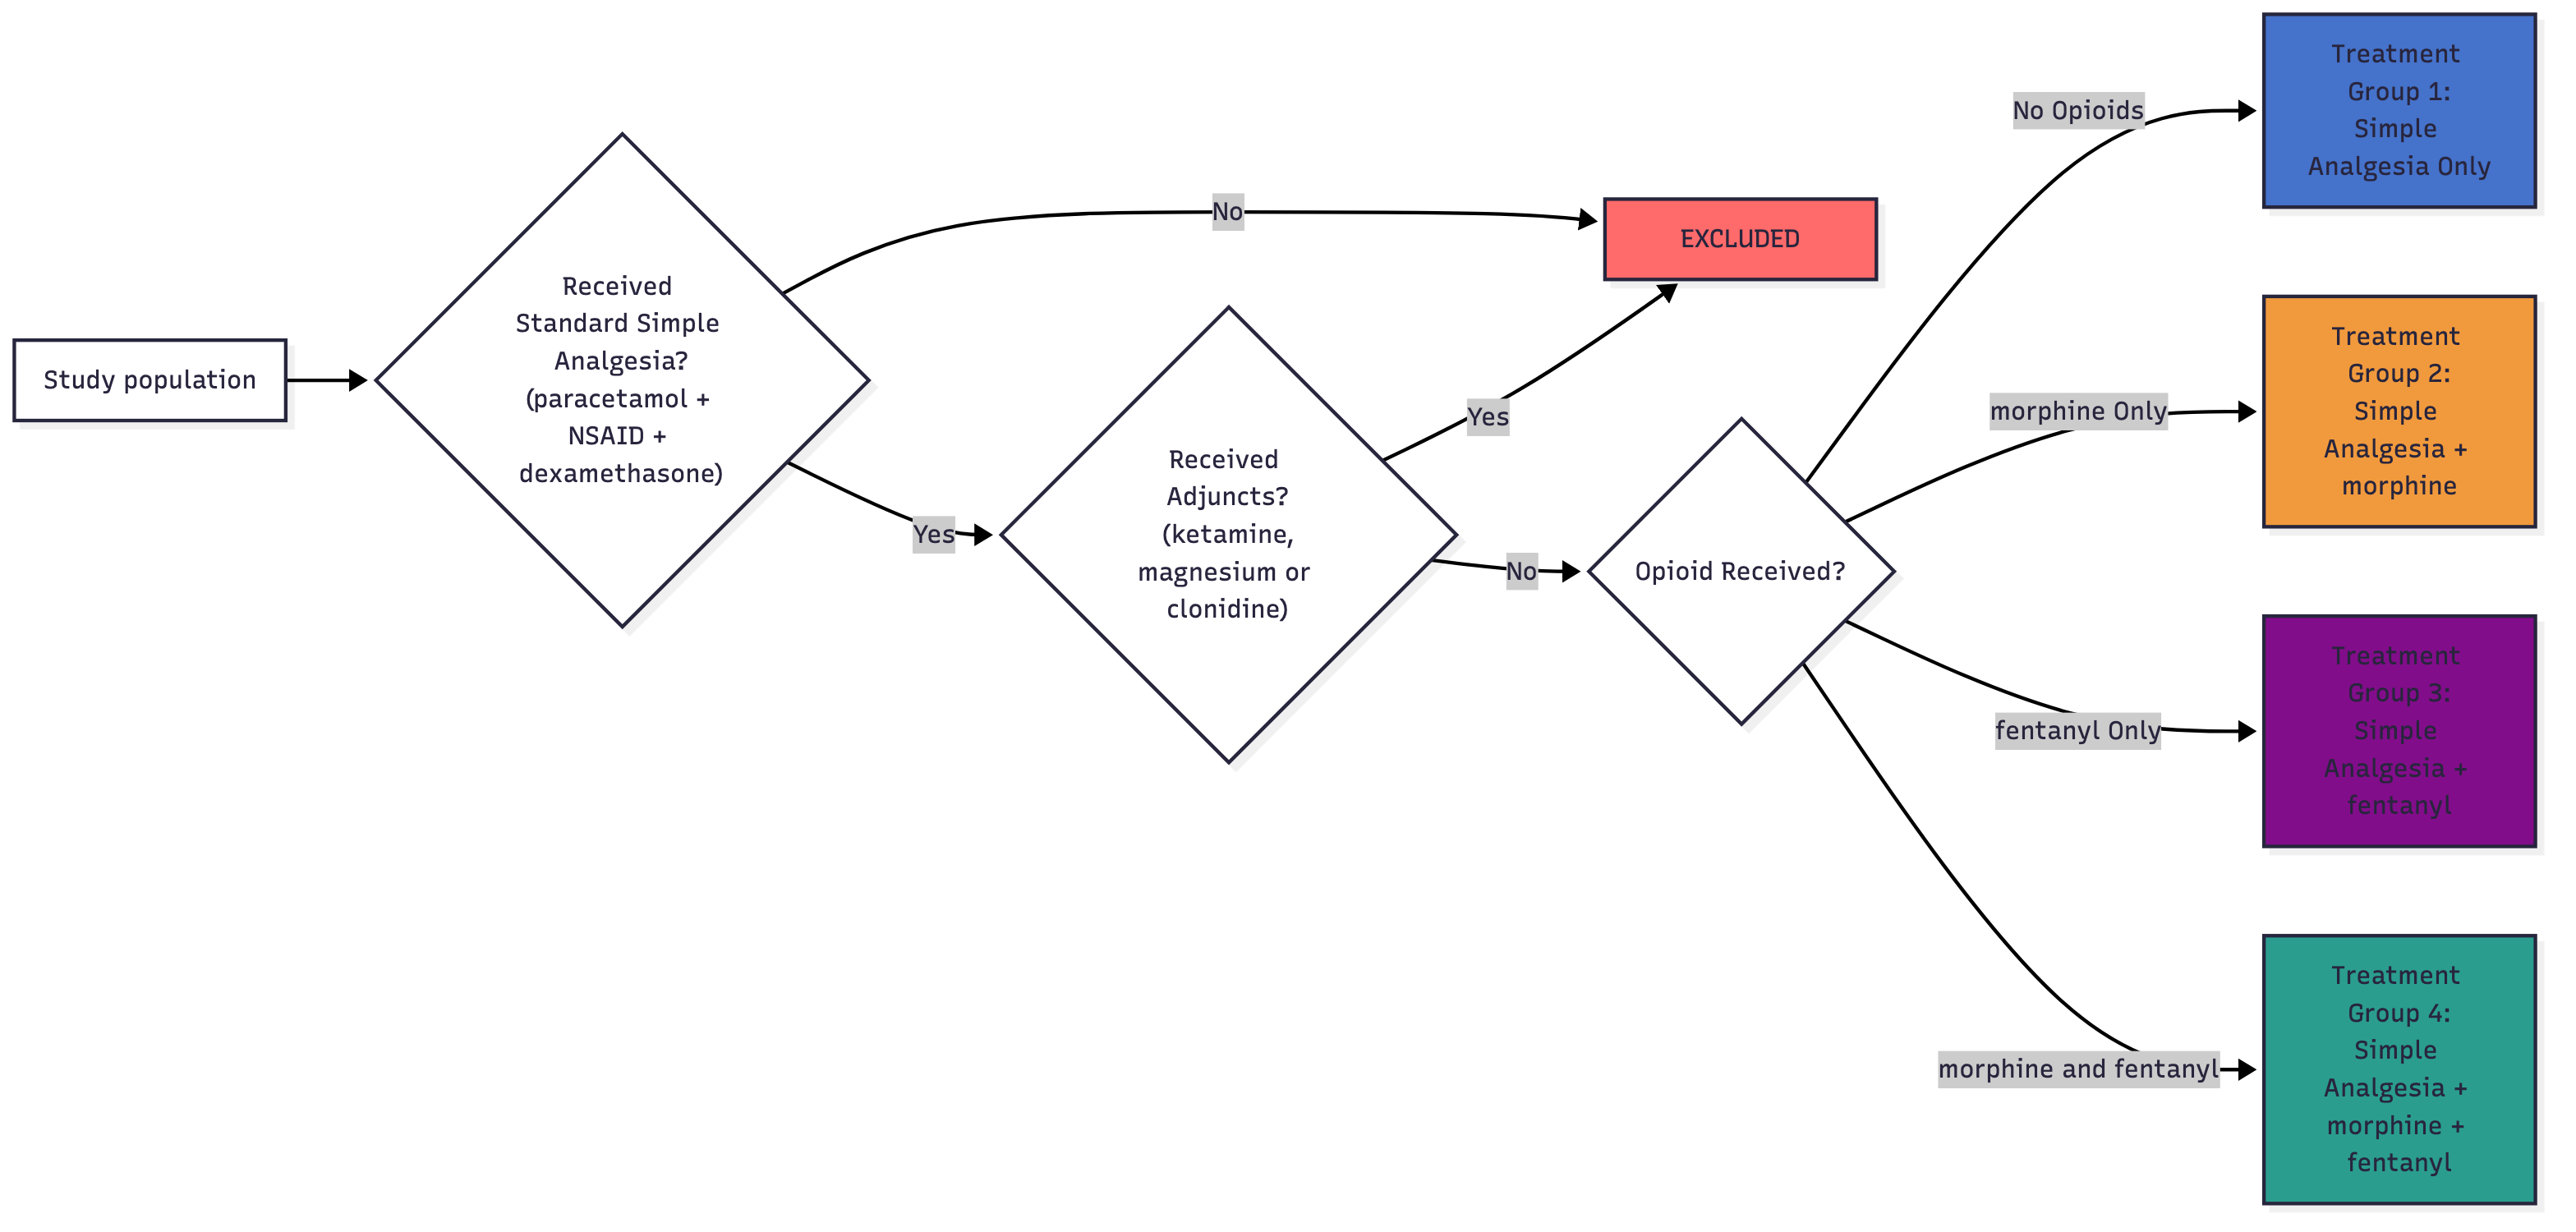
\includegraphics[keepaspectratio]{figures/fig-mermaid-groups.png}}

}

\caption{\label{fig-mermaid-groups}\textbf{Flow chart of treatment group
criteria.} Flowchart describing logic for eligibility for the treatment
groups depending on the medications received.}

\end{figure}%

\subsection{Outcome Measures}\label{outcome-measures}

The primary outcome measure was rescue opioid medication, defined as the
administration of any opioid drug within three hours of the end of the
procedure and recording dose and frequency of administration. This was
chosen as a quantitative measure of intraoperative analgesic
effectiveness during the immediate postoperative period. A sensitivity
analysis was conducted to assess different time cut-offs for opioid
administration within the initial recovery period
(Section~\ref{sec-sm-sensitivity-opioid}). Secondary outcomes were
chosen to reflect a range of process and effectiveness measures directly
relevant to tonsillectomy patients. These were: time spent in
first-stage recovery (a key determinant of patient flow for day case
procedures and influenced by over or under administration of analgesia)
and numerical pain score at rest (0-4) for the first three postoperative
hours. Length of hospital admission was calculated from day of procedure
to hospital discharge. The number and details of opioid prescriptions
for postoperative analgesia on hospital discharge were extracted and
grouped into `weak' or `strong' opioids as per World Health Organisation
definitions (Section~\ref{sec-sm-data-spec-discharge}). Data pertaining
to return to theatre and re-presentation to the UCLH emergency
department within 7, 14 and 30 postoperative days and in-hospital, 30
day and one year mortality were also reported where available.

\subsection{Statistical Analysis}\label{statistical-analysis}

The variables listed were described using absolute numbers (percentages)
for categorical variables, parametrically distributed variables are
shown as means (standard deviations and medians (interquartile ranges)
are presented for non-parametric variables. Descriptions for analgesic
exposure, perioperative analgesic strategy and outcome variables are
presented, stratified by adult and paediatric cohorts, and surgical
subgroups. Multilevel modelling was used to investigate the association
between analgesic strategy the primary and secondary outcomes,
accounting for clinically relevant co-variants selected using expert
domain knowledge and directed acyclic graphs
(Section~\ref{sec-sm-modelling-dag}). Models were constructed for each
outcome measure, with anaesthetic consultant identity incorporated as a
random effect. Where the anaesthetic consultant identifier was not
associated with five or more cases, these were excluded following a
sensitivity analysis (Section~\ref{sec-sm-sensitivity-group-size}).

\section{Results}\label{results-1}

\subsection{Study Population}\label{study-population}

3,656 patients had a surgical encounter matching the predefined OPCS
codes during the study period. Table~\ref{tbl-demo-all} shows the
demographics of both adult and paediatric cohorts.

\begin{table}

\caption{\label{tbl-demo-all}\textbf{Demographics table - All patients.}
Participant baseline demographics and clinical history stratified by
adult and paediatric cohorts. Categorical data as number (\%). IQR
(Interquartile Range), EPR (Electronic Patient Record). Missing data
count and proportion of total cohort presented}

\centering{

\fontsize{12.0pt}{14.4pt}\selectfont
\begin{tabular*}{\linewidth}{@{\extracolsep{\fill}}llll}
\toprule
 &  & Adult cohort & Paediatric cohort \\ 
\midrule\addlinespace[2.5pt]
{Total encounters (\%)} & {} & {1397 (38.2)} & {2259 (61.8)} \\ 
{\cellcolor[HTML]{F2F2F2}{Age (years)}} & {\cellcolor[HTML]{F2F2F2}{Median (IQR)}} & {\cellcolor[HTML]{F2F2F2}{29.00 (23.00 to 38.00)}} & {\cellcolor[HTML]{F2F2F2}{7.00 (5.00 to 10.00)}} \\ 
{Height (cm)} & {Median (IQR)} & {168.47 (162.48 to 176.98)} & {122.98 (110.46 to 140.48)} \\ 
{\cellcolor[HTML]{F2F2F2}{Weight (kg)}} & {\cellcolor[HTML]{F2F2F2}{Median (IQR)}} & {\cellcolor[HTML]{F2F2F2}{74.40 (63.20 to 89.75)}} & {\cellcolor[HTML]{F2F2F2}{24.40 (18.80 to 37.30)}} \\ 
{Sex} & {Female} & {903 (64.6)} & {1002 (44.4)} \\ 
{\cellcolor[HTML]{F2F2F2}{}} & {\cellcolor[HTML]{F2F2F2}{Male}} & {\cellcolor[HTML]{F2F2F2}{494 (35.4)}} & {\cellcolor[HTML]{F2F2F2}{1257 (55.6)}} \\ 
{Gender Identity} & {Female} & {36 (64.3)} & {2 (50.0)} \\ 
{\cellcolor[HTML]{F2F2F2}{}} & {\cellcolor[HTML]{F2F2F2}{Male}} & {\cellcolor[HTML]{F2F2F2}{20 (35.7)}} & {\cellcolor[HTML]{F2F2F2}{2 (50.0)}} \\ 
{Ethnicity} & {White} & {562 (60.2)} & {777 (46.1)} \\ 
{\cellcolor[HTML]{F2F2F2}{}} & {\cellcolor[HTML]{F2F2F2}{Asian}} & {\cellcolor[HTML]{F2F2F2}{103 (11.0)}} & {\cellcolor[HTML]{F2F2F2}{278 (16.5)}} \\ 
 & {Black} & 96 (10.3) & 269 (16.0) \\ 
{\cellcolor[HTML]{F2F2F2}{}} & {\cellcolor[HTML]{F2F2F2}{Mixed}} & {\cellcolor[HTML]{F2F2F2}{56 (6.0)}} & {\cellcolor[HTML]{F2F2F2}{149 (8.8)}} \\ 
 & {Other} & 117 (12.5) & 213 (12.6) \\ 
\bottomrule
\end{tabular*}

}

\end{table}%

Isolated tonsillectomy was the most common procedure in the adult cohort
(n = 1,247, 89.3\%; Table~\ref{tbl-demo-adult}), whilst paediatric
patients predominantly underwent adenotonsillectomy (n = 1,292, 57.2\%;
\quartostblref{stbl-demo-paed}).

\begin{table}

\caption{\label{tbl-demo-adult}\textbf{Demographics table - Adult
patients.} Participant and surgical data for adult cohort stratified by
surgical procedure group. Categorical data as number (\%). IQR
(Interquartile Range), EPR (Electronic Patient Record).}

\centering{

\fontsize{12.0pt}{14.4pt}\selectfont
\begin{tabular*}{\linewidth}{@{\extracolsep{\fill}}llllll}
\toprule
 &  & Tonsillectomy & Adenoidectomy & Adenotonsillectomy & Total \\ 
\midrule\addlinespace[2.5pt]
{Total encounters (\%)} & {} & {1247 (89.3)} & {111 (7.9)} & {39 (2.8)} & {1397} \\ 
{\cellcolor[HTML]{F2F2F2}{Age (years)}} & {\cellcolor[HTML]{F2F2F2}{Median (IQR)}} & {\cellcolor[HTML]{F2F2F2}{29.00 (24.00 to 38.00)}} & {\cellcolor[HTML]{F2F2F2}{27.00 (21.00 to 35.00)}} & {\cellcolor[HTML]{F2F2F2}{27.00 (21.50 to 35.00)}} & {\cellcolor[HTML]{F2F2F2}{29.00 (23.00 to 38.00)}} \\ 
{Height (cm)} & {Median (IQR)} & {167.99 (162.56 to 176.98)} & {170.99 (162.79 to 178.99)} & {163.99 (157.36 to 172.24)} & {168.47 (162.48 to 176.98)} \\ 
{\cellcolor[HTML]{F2F2F2}{Weight (kg)}} & {\cellcolor[HTML]{F2F2F2}{Median (IQR)}} & {\cellcolor[HTML]{F2F2F2}{74.00 (63.00 to 88.45)}} & {\cellcolor[HTML]{F2F2F2}{78.50 (67.25 to 95.50)}} & {\cellcolor[HTML]{F2F2F2}{83.00 (72.00 to 95.00)}} & {\cellcolor[HTML]{F2F2F2}{74.40 (63.20 to 89.75)}} \\ 
{Sex} & {Female} & {806 (64.6)} & {67 (60.4)} & {30 (76.9)} & {903 (64.6)} \\ 
{\cellcolor[HTML]{F2F2F2}{}} & {\cellcolor[HTML]{F2F2F2}{Male}} & {\cellcolor[HTML]{F2F2F2}{441 (35.4)}} & {\cellcolor[HTML]{F2F2F2}{44 (39.6)}} & {\cellcolor[HTML]{F2F2F2}{9 (23.1)}} & {\cellcolor[HTML]{F2F2F2}{494 (35.4)}} \\ 
{Gender Identity} & {Female} & {27 (58.7)} & {6 (85.7)} & {3 (100.0)} & {36 (64.3)} \\ 
{\cellcolor[HTML]{F2F2F2}{}} & {\cellcolor[HTML]{F2F2F2}{Male}} & {\cellcolor[HTML]{F2F2F2}{19 (41.3)}} & {\cellcolor[HTML]{F2F2F2}{1 (14.3)}} & {\cellcolor[HTML]{F2F2F2}{}} & {\cellcolor[HTML]{F2F2F2}{20 (35.7)}} \\ 
{Ethnicity} & {White} & {510 (61.3)} & {38 (47.5)} & {14 (63.6)} & {562 (60.2)} \\ 
{\cellcolor[HTML]{F2F2F2}{}} & {\cellcolor[HTML]{F2F2F2}{Asian}} & {\cellcolor[HTML]{F2F2F2}{86 (10.3)}} & {\cellcolor[HTML]{F2F2F2}{15 (18.8)}} & {\cellcolor[HTML]{F2F2F2}{2 (9.1)}} & {\cellcolor[HTML]{F2F2F2}{103 (11.0)}} \\ 
 & Black & {77 (9.3)} & 16 (20.0) & 3 (13.6) & 96 (10.3) \\ 
{\cellcolor[HTML]{F2F2F2}{}} & {\cellcolor[HTML]{F2F2F2}{Mixed}} & {\cellcolor[HTML]{F2F2F2}{49 (5.9)}} & {\cellcolor[HTML]{F2F2F2}{5 (6.2)}} & {\cellcolor[HTML]{F2F2F2}{2 (9.1)}} & {\cellcolor[HTML]{F2F2F2}{56 (6.0)}} \\ 
 & Other & {110 (13.2)} & 6 (7.5) & 1 (4.5) & 117 (12.5) \\ 
{\cellcolor[HTML]{F2F2F2}{ASA physical status}} & {\cellcolor[HTML]{F2F2F2}{1}} & {\cellcolor[HTML]{F2F2F2}{587 (47.3)}} & {\cellcolor[HTML]{F2F2F2}{56 (50.9)}} & {\cellcolor[HTML]{F2F2F2}{13 (34.2)}} & {\cellcolor[HTML]{F2F2F2}{656 (47.3)}} \\ 
 & 2 & {578 (46.6)} & 46 (41.8) & 22 (57.9) & 646 (46.5) \\ 
{\cellcolor[HTML]{F2F2F2}{}} & {\cellcolor[HTML]{F2F2F2}{3}} & {\cellcolor[HTML]{F2F2F2}{75 (6.0)}} & {\cellcolor[HTML]{F2F2F2}{8 (7.3)}} & {\cellcolor[HTML]{F2F2F2}{3 (7.9)}} & {\cellcolor[HTML]{F2F2F2}{86 (6.2)}} \\ 
{Chronic Tonsillitis EPR Diagnosis} & {Yes} & {905 (72.6)} & {96 (86.5)} & {37 (94.9)} & {1038 (74.3)} \\ 
{\cellcolor[HTML]{F2F2F2}{Obstructive Sleep Apnoea EPR Diagnosis}} & {\cellcolor[HTML]{F2F2F2}{Yes}} & {\cellcolor[HTML]{F2F2F2}{175 (14.0)}} & {\cellcolor[HTML]{F2F2F2}{13 (11.7)}} & {\cellcolor[HTML]{F2F2F2}{13 (33.3)}} & {\cellcolor[HTML]{F2F2F2}{201 (14.4)}} \\ 
{Opioid dependance EPR Diagnosis} & {Yes} & {0 (0.0)} & {0 (0.0)} & {0 (0.0)} & {0 (0.0)} \\ 
{\cellcolor[HTML]{F2F2F2}{Chronic Pain EPR Diagnosis}} & {\cellcolor[HTML]{F2F2F2}{Yes}} & {\cellcolor[HTML]{F2F2F2}{6 (0.5)}} & {\cellcolor[HTML]{F2F2F2}{0 (0.0)}} & {\cellcolor[HTML]{F2F2F2}{0 (0.0)}} & {\cellcolor[HTML]{F2F2F2}{6 (0.4)}} \\ 
{Procedure Length (minutes)} & {Median (IQR)} & {34.00 (24.00 to 48.00)} & {44.00 (23.00 to 66.50)} & {45.00 (33.00 to 58.00)} & {35.00 (25.00 to 49.00)} \\ 
{\cellcolor[HTML]{F2F2F2}{Coblation technique}} & {\cellcolor[HTML]{F2F2F2}{Yes}} & {\cellcolor[HTML]{F2F2F2}{38 (3.0)}} & {\cellcolor[HTML]{F2F2F2}{1 (0.9)}} & {\cellcolor[HTML]{F2F2F2}{4 (10.3)}} & {\cellcolor[HTML]{F2F2F2}{43 (3.1)}} \\ 
\bottomrule
\end{tabular*}

}

\end{table}%

Across all surgical procedures, 1,038 (74.3\%) adults and 2,026 (89.7\%)
children had an EPR diagnosis of chronic tonsillitis. A diagnosis of OSA
was recorded in 201 (14.4\%) adults and 1,241 (54.9\%) children.\\
There was less Coblation use recorded in adult patients compared with
children (n = 43 (3.1\%) and n = 1,344 (59.5\%) respectively).

\subsection{Analgesic Exposure}\label{analgesic-exposure}

All intraoperative analgesic administration is shown in
Table~\ref{tbl-analgesic-adult} (adult) and
\quartostblref{stbl-analgesic-paed} (paediatric) for each surgical
procedure group.

\begin{table}

\caption{\label{tbl-analgesic-adult}\textbf{Anaesthetic management -
Adults.} Intraoperative analgesia administration for adult patients
stratified by surgical group. OME, Oral Morphine Equivalent.}

\centering{

\fontsize{12.0pt}{14.4pt}\selectfont
\begin{tabular*}{\linewidth}{@{\extracolsep{\fill}}llllll}
\toprule
 &  & Tonsillectomy & Adenoidectomy & Adenotonsillectomy & Total \\ 
\midrule\addlinespace[2.5pt]
{Paracetamol (including oral premedications)} & {N (\%)} & {1206 (96.7)} & {102 (91.9)} & {39 (100.0)} & {1347 (96.4)} \\ 
{\cellcolor[HTML]{F2F2F2}{Diclofenac}} & {\cellcolor[HTML]{F2F2F2}{N (\%)}} & {\cellcolor[HTML]{F2F2F2}{1081 (86.7)}} & {\cellcolor[HTML]{F2F2F2}{86 (77.5)}} & {\cellcolor[HTML]{F2F2F2}{35 (89.7)}} & {\cellcolor[HTML]{F2F2F2}{1202 (86.0)}} \\ 
{Dexamethasone} & {N (\%)} & {1228 (98.5)} & {106 (95.5)} & {38 (97.4)} & {1372 (98.2)} \\ 
{\cellcolor[HTML]{F2F2F2}{Clonidine}} & {\cellcolor[HTML]{F2F2F2}{N (\%)}} & {\cellcolor[HTML]{F2F2F2}{38 (3.0)}} & {\cellcolor[HTML]{F2F2F2}{1 (0.9)}} & {\cellcolor[HTML]{F2F2F2}{2 (5.1)}} & {\cellcolor[HTML]{F2F2F2}{41 (2.9)}} \\ 
{Ketamine} & {N (\%)} & {35 (2.8)} & {0 (0.0)} & {0 (0.0)} & {35 (2.5)} \\ 
{\cellcolor[HTML]{F2F2F2}{Magnesium}} & {\cellcolor[HTML]{F2F2F2}{N (\%)}} & {\cellcolor[HTML]{F2F2F2}{83 (6.7)}} & {\cellcolor[HTML]{F2F2F2}{9 (8.1)}} & {\cellcolor[HTML]{F2F2F2}{4 (10.3)}} & {\cellcolor[HTML]{F2F2F2}{96 (6.9)}} \\ 
{Tramadol} & {N (\%)} & {0 (0.0)} & {0 (0.0)} & {0 (0.0)} & {0 (0.0)} \\ 
{\cellcolor[HTML]{F2F2F2}{Oxycodone}} & {\cellcolor[HTML]{F2F2F2}{N (\%)}} & {\cellcolor[HTML]{F2F2F2}{0 (0.0)}} & {\cellcolor[HTML]{F2F2F2}{0 (0.0)}} & {\cellcolor[HTML]{F2F2F2}{0 (0.0)}} & {\cellcolor[HTML]{F2F2F2}{0 (0.0)}} \\ 
{Diamorphine} & {N (\%)} & {0 (0.0)} & {0 (0.0)} & {0 (0.0)} & {0 (0.0)} \\ 
{\cellcolor[HTML]{F2F2F2}{Fentanyl}} & {\cellcolor[HTML]{F2F2F2}{N (\%)}} & {\cellcolor[HTML]{F2F2F2}{833 (66.8)}} & {\cellcolor[HTML]{F2F2F2}{70 (63.1)}} & {\cellcolor[HTML]{F2F2F2}{29 (74.4)}} & {\cellcolor[HTML]{F2F2F2}{932 (66.7)}} \\ 
{Fentanyl, Intraoperative Administration, Dose (µg)} & {Median (IQR)} & {100.00 (100.00 to 150.00)} & {100.00 (100.00 to 100.00)} & {100.00 (100.00 to 200.00)} & {100.00 (100.00 to 150.00)} \\ 
{\cellcolor[HTML]{F2F2F2}{Morphine}} & {\cellcolor[HTML]{F2F2F2}{N (\%)}} & {\cellcolor[HTML]{F2F2F2}{551 (44.2)}} & {\cellcolor[HTML]{F2F2F2}{2 (1.8)}} & {\cellcolor[HTML]{F2F2F2}{12 (30.8)}} & {\cellcolor[HTML]{F2F2F2}{565 (40.4)}} \\ 
{Morphine, Intraoperative Administration, Dose (mg)} & {Median (IQR)} & {10.00 (5.00 to 10.00)} & {5.00 (5.00 to 5.00)} & {8.00 (5.00 to 10.00)} & {10.00 (5.00 to 10.00)} \\ 
{\cellcolor[HTML]{F2F2F2}{Intra-operative opioids given}} & {\cellcolor[HTML]{F2F2F2}{N (\%)}} & {\cellcolor[HTML]{F2F2F2}{1139 (91.3)}} & {\cellcolor[HTML]{F2F2F2}{72 (64.9)}} & {\cellcolor[HTML]{F2F2F2}{39 (100.0)}} & {\cellcolor[HTML]{F2F2F2}{1250 (89.5)}} \\ 
{Total intraoperative opioid dose  (OME, mg)} & {Median (IQR)} & {30.00 (20.00 to 40.00)} & {20.00 (20.00 to 20.00)} & {30.00 (20.00 to 37.50)} & {30.00 (20.00 to 40.00)} \\ 
{\cellcolor[HTML]{F2F2F2}{Treatment group}} & {\cellcolor[HTML]{F2F2F2}{1}} & {\cellcolor[HTML]{F2F2F2}{76 (8.1)}} & {\cellcolor[HTML]{F2F2F2}{27 (36.0)}} & {\cellcolor[HTML]{F2F2F2}{0 (0.0)}} & {\cellcolor[HTML]{F2F2F2}{103 (9.9)}} \\ 
 & 2 & {232 (24.7)} & 1 (1.3) & 8 (26.7) & 241 (23.1) \\ 
{\cellcolor[HTML]{F2F2F2}{}} & {\cellcolor[HTML]{F2F2F2}{3}} & {\cellcolor[HTML]{F2F2F2}{448 (47.7)}} & {\cellcolor[HTML]{F2F2F2}{47 (62.7)}} & {\cellcolor[HTML]{F2F2F2}{21 (70.0)}} & {\cellcolor[HTML]{F2F2F2}{516 (49.4)}} \\ 
 & 4 & {183 (19.5)} & 0 (0.0) & 1 (3.3) & 184 (17.6) \\ 
\bottomrule
\end{tabular*}

}

\end{table}%

\subsubsection{Simple Analgesia -- Paracetamol, NSAID,
Dexamethasone}\label{simple-analgesia-paracetamol-nsaid-dexamethasone}

Across the adult population, 82.9\% (n = 1,158) of patients received a
standard simple analgesia combination of paracetamol, diclofenac and
dexamethasone (Figure~\ref{fig-venn-adult} (A)). Of those that did not
receive all three medications, the most common omission was diclofenac
(Figure~\ref{fig-venn-adult} (B)). In the paediatric cohort 72.0\% (n =
1,627) of patients received complete simple analgesia
(\quartosfigref{sfig-venn-paed} (A)).\\
Paracetamol was given in 98.8\% (n = 2,232) of paediatric cases, of
which 20.2\% (n = 456) was received as an oral dose prior to theatre
(\quartosfigref{sfig-venn-paed} (B)). Oral pre-dosing was not common in
the adult cohort (4.7\%, n = 65), but overall perioperative use was
similarly high (96.4\%, n = 1,347). There was no use of selective COX-2
inhibitor drugs during the study period.

\begin{figure}[H]

\centering{

\pandocbounded{\includegraphics[keepaspectratio,alt={Venn diagrams of adult intraoperative medications}]{manuscript_files/figure-pdf/fig-venn-adult-1.pdf}}

}

\caption{\label{fig-venn-adult}\textbf{Venn diagrams of adult
intraoperative medications.} Distributions of complete intra-operative
simple analgesia and intraoperative opioid administration in adults (A).
Venn diagram to show the breakdown of the simple analgesia (B) and
opioids given (C)}

\end{figure}%

\subsubsection{Opioid Analgesia}\label{opioid-analgesia}

89.5\% (n = 1,250) of adult patients and 98.3\% (n = 2,221) of
paediatric patients received a strong opioid medication intraoperatively
(Section~\ref{sec-sm-data-spec-intra-op-meds}).
Table~\ref{tbl-analgesic-adult} (adult) and
\quartostblref{stbl-analgesic-paed} (paediatric) show the breakdown of
opioid medication use across each surgical procedure group.\\
Across all procedures, a single opioid strategy with fentanyl was most
common in children, accounting for 95.4\% of cases (n = 2,156;
\quartosfigref{sfig-venn-paed} C). Adults received a mix of strategies,
with 49.0\% (n = 685) receiving fentanyl only, 22.8\% (n = 318) morphine
only, 17.7\% (n = 247) receiving both and 10.5\% (n = 147) receiving
neither, illustrated in Figure~\ref{fig-venn-adult} C). The median
intraoperative opioid dose administered to adults was 30mg (OME, IQR =
20-40mg). Patients receiving a regimen of simple analgesia plus morphine
only received a median 30mg OME (IQR 15-30mg), contrasting with 20mg OME
(IQR 20-30mg) in fentanyl only group, and 50mg (IQR 41-50mg) in the
combined opioid group (\quartosfigref{sfig-opioid-histogram-adult}).
Paediatric patients received a median fentanyl dose of 1.14 mcg.kg-1
(IQR = 0.99 -- 1.85 mcg.kg-1) and a median morphine dose of 0.10 mg.kg-1
(IQR = 0.06 -- 0.10 mg.kg-1).

No patients received oxycodone, diamorphine or tramadol
intraoperatively.

\subsubsection{Non-Opioid Analgesics -- Clonidine, Ketamine,
Magnesium}\label{non-opioid-analgesics-clonidine-ketamine-magnesium}

The use of non-opioid analgesics was generally low across both adult and
paediatric cohorts (\quartosfigref{sfig-venn-adjuncts}). 4.3\% (n = 157)
of patients received either clonidine, ketamine and or magnesium.
Clonidine was used in 2.9\% (n = 41) of adult cases and 0.1\% (n = 3) of
paediatric cases, whilst ketamine was used in 2.5\% (n = 35) of adult
cases and 0.0\% (n = 1) of paediatric cases. Magnesium was used in 6.9\%
(n = 96) adult cases and 0.2\% (n = 4) paediatric cases.

\subsubsection{Combined Analgesic
Strategies}\label{combined-analgesic-strategies}

Across the adult cohort, the most common analgesic combination seen was
Group 3 (n = 516, 36.9\% of all adult patients), followed by Group 2 (n
= 241, 17.3\%) and Group 4 (n = 184,
13.2\%)(Table~\ref{tbl-analgesic-adult}). Figure~\ref{fig-upset-adult}
shows the relative distribution of the different possible combinations
of intraoperative analgesic agents.

\begin{figure}[H]

\centering{

\includegraphics[width=10in,height=\textheight,keepaspectratio,alt={UpSet graph of the combinations of adult intraoperative analgesia}]{data/upset_adult.png}

}

\caption{\label{fig-upset-adult}\textbf{UpSet graph of the combinations
of adult intraoperative analgesia.} Distribution of the different
analgesic combinations for adults patients. Upper vertical bar graph
showing the total count of each combination of analgesia with treatment
groups coloured. Lower left horizontal bar graph showing the total count
of patients receiving each specific medication.}

\end{figure}%

Across the paediatric cohort less heterogeneity in the analgesic
combinations was observed (\quartosfigref{sfig-upset-paed}). The
commonest strategy was Group 3 (n = 1,538, 68.1\%), followed by Group 4
(n = 52, 2.3\%). 28.0\% (n = 632) of the paediatric cohort did not
receive a complete combination of simple analgesia (paracetamol, NSAID
and dexamethasone).

\subsection{Outcomes}\label{outcomes}

Across all surgical procedure groups, 55.7\% (n = 778) of adult patients
required rescue opioid administration in the first three postoperative
hours, compared to 4.0\% (n = 90) of children. In adults, the median
dose of rescue opioid administered was 20mg (OME, IQR = 12.0-20mg), of
which 98\% was administered as fentanyl (n = 762). The breakdown of
administration across each surgical procedure group and secondary
outcome measures are shown in Table~\ref{tbl-outcome-adult} (adult) and
\quartostblref{stbl-outcome-paed} (paediatric).

\begin{table}

\caption{\label{tbl-outcome-adult}\textbf{Adult outcomes.} Outcome data
for adult patients stratified by surgical group. Return to theatre at
UCLH and representation to UCLH emergency department only, cumulative
measures at each time point. Eligible medications for discharge measured
as classified in Section~\ref{sec-sm-data-spec}.}

\centering{

\fontsize{12.0pt}{14.4pt}\selectfont
\begin{tabular*}{\linewidth}{@{\extracolsep{\fill}}llllll}
\toprule
 &  & Tonsillectomy & Adenoidectomy & Adenotonsillectomy & Total \\ 
\midrule\addlinespace[2.5pt]
{Administration of rescue opioids} & {N (\%)} & {709 (56.9)} & {45 (40.5)} & {24 (61.5)} & {778 (55.7)} \\ 
{\cellcolor[HTML]{F2F2F2}{Administration of rescue morphine}} & {\cellcolor[HTML]{F2F2F2}{N (\%)}} & {\cellcolor[HTML]{F2F2F2}{23 (1.8)}} & {\cellcolor[HTML]{F2F2F2}{0 (0.0)}} & {\cellcolor[HTML]{F2F2F2}{0 (0.0)}} & {\cellcolor[HTML]{F2F2F2}{23 (1.6)}} \\ 
{Administration of rescue fentanyl} & {N (\%)} & {693 (55.6)} & {45 (40.5)} & {24 (61.5)} & {762 (54.5)} \\ 
{\cellcolor[HTML]{F2F2F2}{Administration of rescue opioids, (OME mg)}} & {\cellcolor[HTML]{F2F2F2}{Median (IQR)}} & {\cellcolor[HTML]{F2F2F2}{20.00 (12.00 to 20.00)}} & {\cellcolor[HTML]{F2F2F2}{20.00 (12.00 to 20.00)}} & {\cellcolor[HTML]{F2F2F2}{20.00 (12.00 to 20.00)}} & {\cellcolor[HTML]{F2F2F2}{20.00 (12.00 to 20.00)}} \\ 
{Time in Stage 1 recovery (mins)} & {Median (IQR)} & {71.00 (46.36 to 102.68)} & {65.18 (40.81 to 90.11)} & {77.63 (62.19 to 98.97)} & {70.97 (46.16 to 101.41)} \\ 
{\cellcolor[HTML]{F2F2F2}{Pain score at rest 3hrs post-op (Median)}} & {\cellcolor[HTML]{F2F2F2}{Median (IQR)}} & {\cellcolor[HTML]{F2F2F2}{1.00 (0.00 to 2.00)}} & {\cellcolor[HTML]{F2F2F2}{0.50 (0.00 to 1.00)}} & {\cellcolor[HTML]{F2F2F2}{1.00 (0.00 to 2.00)}} & {\cellcolor[HTML]{F2F2F2}{1.00 (0.00 to 2.00)}} \\ 
{Length of Stay (days)} & {Median (IQR)} & {0.44 (0.38 to 0.56)} & {0.36 (0.30 to 0.44)} & {0.42 (0.37 to 0.76)} & {0.43 (0.38 to 0.55)} \\ 
{\cellcolor[HTML]{F2F2F2}{Same day discharge}} & {\cellcolor[HTML]{F2F2F2}{N (\%)}} & {\cellcolor[HTML]{F2F2F2}{951 (76.3)}} & {\cellcolor[HTML]{F2F2F2}{92 (82.9)}} & {\cellcolor[HTML]{F2F2F2}{29 (74.4)}} & {\cellcolor[HTML]{F2F2F2}{1072 (76.7)}} \\ 
{Paracetamol on discharge} & {N (\%)} & {643 (51.6)} & {12 (10.8)} & {25 (64.1)} & {680 (48.7)} \\ 
{\cellcolor[HTML]{F2F2F2}{NSAID on discharge}} & {\cellcolor[HTML]{F2F2F2}{N (\%)}} & {\cellcolor[HTML]{F2F2F2}{770 (61.7)}} & {\cellcolor[HTML]{F2F2F2}{11 (9.9)}} & {\cellcolor[HTML]{F2F2F2}{25 (64.1)}} & {\cellcolor[HTML]{F2F2F2}{806 (57.7)}} \\ 
{Strong opioid perscribed on discharge} & {N (\%)} & {19 (1.5)} & {0 (0.0)} & {0 (0.0)} & {19 (1.4)} \\ 
{\cellcolor[HTML]{F2F2F2}{New strong opioids on discharge}} & {\cellcolor[HTML]{F2F2F2}{N (\%)}} & {\cellcolor[HTML]{F2F2F2}{0 (NaN)}} & {\cellcolor[HTML]{F2F2F2}{0 (NaN)}} & {\cellcolor[HTML]{F2F2F2}{0 (NaN)}} & {\cellcolor[HTML]{F2F2F2}{0 (NaN)}} \\ 
{Weak opioid on discharge} & {N (\%)} & {1070 (85.8)} & {23 (20.7)} & {31 (79.5)} & {1124 (80.5)} \\ 
{\cellcolor[HTML]{F2F2F2}{Return to theatre within 7 days}} & {\cellcolor[HTML]{F2F2F2}{N (\%)}} & {\cellcolor[HTML]{F2F2F2}{7 (0.6)}} & {\cellcolor[HTML]{F2F2F2}{0 (0.0)}} & {\cellcolor[HTML]{F2F2F2}{0 (0.0)}} & {\cellcolor[HTML]{F2F2F2}{7 (0.5)}} \\ 
{Return to theatre within 14 days} & {N (\%)} & {15 (1.2)} & {0 (0.0)} & {0 (0.0)} & {15 (1.1)} \\ 
{\cellcolor[HTML]{F2F2F2}{Return to theatre within 30 days}} & {\cellcolor[HTML]{F2F2F2}{N (\%)}} & {\cellcolor[HTML]{F2F2F2}{19 (1.5)}} & {\cellcolor[HTML]{F2F2F2}{0 (0.0)}} & {\cellcolor[HTML]{F2F2F2}{0 (0.0)}} & {\cellcolor[HTML]{F2F2F2}{19 (1.4)}} \\ 
{Represented to ED before 7 days} & {N (\%)} & {167 (13.4)} & {4 (3.6)} & {2 (5.1)} & {173 (12.4)} \\ 
{\cellcolor[HTML]{F2F2F2}{Represented to ED before 14 days}} & {\cellcolor[HTML]{F2F2F2}{N (\%)}} & {\cellcolor[HTML]{F2F2F2}{229 (18.4)}} & {\cellcolor[HTML]{F2F2F2}{8 (7.2)}} & {\cellcolor[HTML]{F2F2F2}{6 (15.4)}} & {\cellcolor[HTML]{F2F2F2}{243 (17.4)}} \\ 
{Represented to ED before 30 days} & {N (\%)} & {235 (18.8)} & {9 (8.1)} & {6 (15.4)} & {250 (17.9)} \\ 
{\cellcolor[HTML]{F2F2F2}{Died during admission}} & {\cellcolor[HTML]{F2F2F2}{N (\%)}} & {\cellcolor[HTML]{F2F2F2}{1 (0.1)}} & {\cellcolor[HTML]{F2F2F2}{0 (0.0)}} & {\cellcolor[HTML]{F2F2F2}{0 (0.0)}} & {\cellcolor[HTML]{F2F2F2}{1 (0.1)}} \\ 
{Mortality (90 days)} & {N (\%)} & {1 (0.1)} & {0 (0.0)} & {0 (0.0)} & {1 (0.1)} \\ 
{\cellcolor[HTML]{F2F2F2}{Mortality (1 year)}} & {\cellcolor[HTML]{F2F2F2}{N (\%)}} & {\cellcolor[HTML]{F2F2F2}{4 (0.4)}} & {\cellcolor[HTML]{F2F2F2}{0 (0.0)}} & {\cellcolor[HTML]{F2F2F2}{0 (0.0)}} & {\cellcolor[HTML]{F2F2F2}{4 (0.3)}} \\ 
\bottomrule
\end{tabular*}

}

\end{table}%

Adults spent a median 71.0 minutes (IQR = 46.2 -- 101.4 minutes) in
first stage recovery, with 76.7\% (n = 1,072) going to be discharged
home the same day. The median length of stay from admission to hospital
discharge was 0.43 days (IQR = 0.38-0.55). Most adults (80.5\%, n =
1,124) received a weak opioid prescription on discharge. 19 (1.4\%)
adult patients received a strong opioid prescription on discharge, all
of which were continuations of an existing preoperative opioid
prescription. There were no newly initiated strong opioid prescriptions.
Children spent a median 27.6 minutes (IQR = 18.6 -- 37.5 minutes) in
first stage recovery, with 94.4\% (n = 2,132) going on to be discharged
the same day. 33.6\% (n = 760) were discharged with paracetamol, 30.9\%
(n = 699) with an NSAID, with 33 (1.5\%) receiving a weak opioid
prescription and 5 (0.2\%) receiving a strong opioid prescription; of
which all were a continuation of a pre-admission strong opioid.\\
Rates of return to theatre were low with 1.4\% (n = 19) of adults and
0.3\% (n = 7) paediatric cases returning within 30 days. 1 adult patient
died during the surgical encounter. Across the whole study sample, the
representation rate to the study centre's emergency department (ED)
within 30 days was 10.4\% (n = 380), 17.9\% (n = 250) in adults and
5.8\% (n = 130) in children. A manual review of 50 randomly selected
cases representing to the ED showed that 52\% (n =26) were related to
bleeding, 38\% (n = 19) related to pain control, 4\% (n = 2) with
symptoms of infection. Three patients represented for reasons unrelated
to surgery. Of the 50 cases reviewed, 55\% (n = 26) were admitted to
hospital for further treatment.

\subsection{Association of Analgesic Strategy with
Outcomes}\label{association-of-analgesic-strategy-with-outcomes}

For the primary outcome measure, unadjusted (rescue analgesia and
analgesic group) and adjusted models (incorporating clinically relevant
covariates as fixed effects) are presented.
\quartosfigref{sfig-consort-modelling} shows the composition of adult
and paediatric cohorts used for model construction and the distribution
of the associated treatment groups. Given the lack of observed variation
in the analgesic and opioid practices for the paediatric cohort, this
analysis was confined to the adult cohort.

\subsubsection{Adults}\label{adults}

After applying exclusion criteria, 975 patients were included in the
analysis. The most common analgesic group was 3 (n = 474, 48.6\%),
followed by 2 (n = 232, 23.8\%), 4 (n = 170, 17.4\%) and 1 (n = 99,
10.2\%).\\
An unadjusted generalised linear mixed effects model (model 1) examining
the association of rescue opioid administration with analgesic group
(using group 1 as a reference) and nested by anaesthetic consultant
identity demonstrated a 63.3\% chance of receiving rescue opioids in
recovery for patients who did not receive any intraoperative opioid
(group 1). Group 4 (simple analgesia plus morphine and fentanyl)
demonstrated a significant negative association (OR 0.283, 95\% CI
0.165-0.486). Anaesthetist identity accounted for 5.0\% (SD 22\%) of the
observed variation in the unadjusted model.\\
After adjusting for age, sex, surgical procedure type, ASA, chronic pain
history, procedure length, use of a Coblation technique and
intraoperative opioid dose (model 2), the association observed for Group
4 was no longer significant (OR 0.418, 95\% CI 0.16-1.09). Variation
associated with the individual anaesthetist was 4.1\% (SD 20\%).

The same model parameters were used to evaluate the secondary outcomes
(\quartosfigref{sfig-forrest-plot}). Treatment group 4 showed a reduced
time in recovery (-42.1 minutes, 95\% CI -66.7 to -17.5) and an
increased, but not significant, odds ratio of 3.17 of same day discharge
(95\% CI 0.961 to 10.5). Modelling of pain scores was not possible due
to the lack of distribution in data and the model of presentations to
the emergency department was non-significant with low confidence
(Section~\ref{sec-sm-modelling}).

\section{Discussion}\label{discussion}

This single-centre, retrospective EPR cohort study investigated the
intraoperative use of opioid medications in adult and paediatric
patients undergoing tonsillectomy and adenotonsillectomy. Using
routinely collected electronic patient data for 3,656 patients we were
able to examine patient, surgical and anaesthetic variables relating to
perioperative analgesic management and intraoperative opioid
administration. The majority of patients (76.2\%, n = 2,785) received
the combination of simple analgesia recommended by the current PROSPECT
guidelines (paracetamol, NSAID, and dexamethasone). Additionally, 94.9\%
of adults and children received an intraoperative opioid medication. In
children, most (95.4\%, n = 2,156) received a single opioid regimen of
fentanyl, at a median dose of 1.14 mcg.kg-1 (IQR 0.99-1.85 mcg.kg-1).
Opioid strategies in adults were less uniform, with 49.0\% (n = 685)
receiving a fentanyl-only strategy, 22.8\% (n = 318) receiving morphine
only, and 17.7\% (n = 247) receiving both.

To investigate the association between opioid technique and immediate
postoperative outcomes, patients were categorised into one of four
treatment groups based on the receipt of full simple analgesia, simple
analgesia plus a single opioid (fentanyl or morphine) and simple
analgesia plus both opioid medications. Patients who received additional
non-opioid analgesia were excluded. Due to the lack of opioid variation
in the paediatric cohort this analysis was confined to adults. Patients
in the combined opioid group received a higher median dose (50mg
vs.~20mg vs.~30mg OME) compared with the morphine and fentanyl-only
groups respectively, indicating clinicians had different dosing
strategies in addition to opioid preferences.

Multilevel modelling, accounting for the individual anaesthetic
consultant and adjusting for a range of clinically relevant patient,
surgical and anaesthetic covariates revealed no statistically
significant association between type of opioid and receipt of rescue
analgesia in the first three postoperative hours compared to the simple
analgesia only group. However, the fentanyl-only (23.4 minutes 95\% CI
6.8 -- 40.0) and combined opioid groups (42.1 minutes, 95\% CI 17.5 --
66.7) were associated with less time in recovery. In addition, the
morphine only group was associated with better odds of being discharged
home on the day of surgery (Group 2 OR 2.27, 1.02-5.06), potentially
suggesting that fentanyl is effective in the short-term, but a
morphine-containing opioid strategy may have benefits extending beyond
the initial recovery period. Intraoperative opioid treatment group was
not associated with chance of receiving a strong opioid prescription on
discharge from hospital, or representation to the hospitals' ED in the
first seven postoperative days. Given that tonsillectomy and
adenotonsillectomy are associated with high rates of representation
compared with other day case procedures Powell et al. (2026), this
suggests intraoperative opioid strategy is unlikely to influence pain
control in the days following surgery.

In general, there is a lack of evidence supporting the optimal
intraoperative analgesic strategy for both and adult and paediatric
tonsillectomy. Most focuses on the safety and effectiveness of
postoperative analgesia, or the evaluation of specific intraoperative
agents and techniques, such as intracapsular drug infiltration(Dal et
al. 2007; Teunkens et al. 2019; Akkaya et al. 2009), or intravenous
methadone. Bøndergaard M et al. (2025) Whilst the prevailing zeitgeist
appears to be towards opioid minimisation, or opioid free techniques,
responding to concerns around side effects such as postoperative nausea
and vomiting, sedation, or tolerance and hyperalgesia associated with
ultra-short acting agents like remifentanil, there remains little
evidence of what is most effective. Shanthanna et al. (2021) Our
findings suggest that anaesthetists in both adult and paediatric
routinely use opioids intraoperatively, but there is variation in how
these medications are used, particularly in adults.

Bøndergaard and colleagues examined the effectiveness of intravenous
methadone (24-48 hour half-life) versus 3 mcg.kg-1 fentanyl administered
on induction of anaesthesia. Their randomised trial of 120 adult
patients undergoing elective bilateral tonsillectomy revealed lower
immediate postoperative opioid requirements across the first five
postoperative days. There were no between group differences in sedation
or time to discharge, however the methadone group was associated with
significantly higher rates of postoperative nausea and vomiting.
(\textbf{bondergaardIntraoperativeMethadonePostoperative2025?}) We found
no studies directly comparing the effectiveness and safety of
intraoperative morphine and fentanyl regimens in adult patients. Given
these are the two most commonly used intraoperative opioid analgesic
agents in the UK (excluding the use of remifentanil for its lack of
postoperative analgesic benefit), it would make sense to identify the
optimal treatment choice here. Our study results raise the interesting
question as to the potential superiority of a dual analgesic approach,
combining both fentanyl and morphine. In a recent large study by Santa
Cruz Mercardo et al, higher intraoperative opioid administration was
also associated with lower immediate and long term opioid use
postoperatively. Santa Cruz Mercado et al. (2023)

This dual approach might harness the relative differences in time taken
to reach peak effect site concentration for each agent (fentanyl: rapid
onset of action, duration of effect 30-45min; morphine: 15-30min onset
time, 4-6 hour duration of action). Fentanyl is frequently used as a
co-induction agent, to facilitate airway placement and blunt the initial
response to surgery, with morphine being delivered later during the
procedure to provide both intra- and postoperative analgesia. This
rational should apply equally to the combined use of remifentanil and
morphine, which may have been captured in Treatment Group 2. It is
possible that the difference in effect observed between groups 2 and 4
might relate to use of remifentanil, resulting in postoperative
hyperalgesia. The benefit of an intraoperative opioid strategy which
incorporates this concept of pharmacokinetic layering has, to the
authors' knowledge, yet to be examined in this surgical group.

Our study has several strengths. We have demonstrated the practicality
of using a data ecosystem and study pipeline specifically designed to
reduce the barriers to using highly granular, routinely collected
electronic patient data to map current and historical practice and
address specific questions around care variation and treatment
effectiveness. This pipeline is sustainable and will support repeated
analyses as the eligible population continues to grow over time.

By using structured EPR data, we have been able to include variables
relevant to perioperative analgesic management, but which are often
difficult to include in observational studies of this type. These
include patient (pre-existing chronic pain or opioid use), surgical
(procedure length, use of Coblation technique) and anaesthetic (intra-
and postoperative analgesic use) specific variables. By incorporating
these with the individual anaesthetist's preferences using a multilevel
modelling approach, we can move closer to a fuller picture of clinical
decision making for smaller patient subgroups. Finally, the application
of these principles to a large dataset of over 3,000 patients may help
address some of the deficiencies inherent to a retrospective
observational approach.

There are important limitations to this study. This is a single centre
study and despite the relatively large sample size compared with similar
work, this limits the generalisability of our findings. EPR-based
studies are at high risk of bias through several mechanisms. Despite
capturing relevant variables in greater detail than previously possible
in similar work 7, there remain key components missing. In particular,
patient data such as ethnicity was associated with a significant degree
of missingness (Section~\ref{sec-sm-missing-data}). In addition, it was
not possible to reliably determine anaesthetic technique, in particular,
discerning between volatile and total intravenous techniques, which may
significantly influence both the intraoperative opioid administration
practice and postoperative recovery. Finally, whilst the use of
Coblation was reliably coded via a specific procedure code
(Section~\ref{sec-sm-data-spec-procedures}), alternative surgical
approaches such as blunt dissection, or diathermy were not coded,
existing only as unstructured data within the operation record. Further,
there are additional variables relating to surgical technique which are
also unstructured and were not included in the analysis, such as the
extent of surgical dissection (intra versus extra-capsular), which will
also influence postoperative pain and recovery, a limitation noted in
previous studies. Keltie et al. (2021)

Given the lack of accounting for unmeasured confounding using a
multilevel modelling approach, we make no causal judgements on the
associations described. We also acknowledge limitations in our outcome
measures, in particular the imposition of a 3-hour time cut for rescue
opioid administration, given there is no defined transition point
between phases of recovery. A sensitivity analysis exploring different
time cut-offs for defining rescue opioid administration can be found in
Section~\ref{sec-sm-sensitivity-opioid}. Further, we were only able to
capture re-presentation to the study centres' ED. Reported figures are
therefore likely an underestimate as they do not reflect patients
presenting to other hospitals or primary care. Future work should focus
on addressing these limitations. In particular, improving quality of
intraoperative and outcome data as described. Given the subjective
nature of both pain descriptors and recovery from surgery, patient
reported outcome measures should also be defined and incorporated into
future analyses. The lack of clear answer on optimal intraoperative
analgesic technique should also form the basis of future randomised
trials going forward.

In conclusion, adult and paediatric tonsillectomy and adenotonsillectomy
patients in this cohort study commonly received an intraoperative
opioid, in the absence of evidence-based guidance on the optimal
intraoperative opioid strategy. Whilst opioid use in paediatric patients
was uniform, adults showed greater variation, with a corresponding
association to variation in immediate postoperative outcomes after
correcting for key patient, surgical and anaesthetic variables.

\bookmarksetup{startatroot}

\chapter*{References}\label{references}
\addcontentsline{toc}{chapter}{References}

\markboth{References}{References}

\protect\phantomsection\label{refs}
\begin{CSLReferences}{1}{1}
\bibitem[\citeproctext]{ref-akkayaComparisonIntravenousPeritonsillar2009}
Akkaya, Taylan, Nurdan Bedirli, Tijen Ceylan, et al. 2009. {``Comparison
of Intravenous and Peritonsillar Infiltration of Tramadol for
Postoperative Pain Relief in Children Following Adenotonsillectomy:''}
\emph{European Journal of Anaesthesiology} 26 (4): 333--37.
\url{https://doi.org/10.1097/EJA.0b013e32831c8988}.

\bibitem[\citeproctext]{ref-aldamlujiPROSPECTGuidelineTonsillectomy2021}
Aldamluji, N., A. Burgess, E. Pogatzki-Zahn, J. Raeder, H. Beloeil, and
PROSPECT Working Group collaborators*. 2021. {``{PROSPECT} Guideline for
Tonsillectomy: Systematic Review and Procedure-Specific Postoperative
Pain Management Recommendations.''} \emph{Anaesthesia} 76 (7): 947--61.
\url{https://doi.org/10.1111/anae.15299}.

\bibitem[\citeproctext]{ref-bondergaardmIntraoperativeMethadonePostoperative2025}
Bøndergaard M, Uhrbrand PG, Karaca T, et al. 2025. {``Intraoperative
Methadone for Postoperative Pain in Adult Patients Undergoing
Tonsillectomy-a Randomised Controlled Trial.''} \emph{BJA Open}
(England) 14: 100418. \url{https://doi.org/10.1016/j.bjao.2025.100418}.

\bibitem[\citeproctext]{ref-dalEfficacyIntravenousPeritonsillar2007}
Dal, Didem, Nalan Celebi, Elvan Gaye Elvan, Varol Celiker, and Ulku
Aypar. 2007. {``The Efficacy of Intravenous or Peritonsillar
Infiltration of Ketamine for Postoperative Pain Relief in Children
Following Adenotonsillectomy{\textsuperscript{1}}.''} \emph{Pediatric
Anesthesia} 17 (3): 263--69.
\url{https://doi.org/10.1111/j.1460-9592.2006.02095.x}.

\bibitem[\citeproctext]{ref-ENTUKTonsillectomy}
ENT UK. 2021. \emph{Tonsillectomy Commissioning Guide}. The Royal
College of Surgeons, 38-43 Lincoln's Inn Fields, London WC2A 3PE.

\bibitem[\citeproctext]{ref-gerbershagenPainIntensityFirst2013}
Gerbershagen, Hans J., Sanjay Aduckathil, Albert J. M. Van Wijck, Linda
M. Peelen, Cor J. Kalkman, and Winfried Meissner. 2013. {``Pain
{Intensity} on the {First Day} After {Surgery}: {A Prospective Cohort
Study Comparing} 179 {Surgical Procedures}.''} \emph{Anesthesiology} 118
(4): 934--44. \url{https://doi.org/10.1097/ALN.0b013e31828866b3}.

\bibitem[\citeproctext]{ref-keltiePaediatricTonsillectomyEngland2021}
Keltie, Kim, Adam Donne, Mat Daniel, et al. 2021. {``Paediatric
Tonsillectomy in {England}: {A} Cohort Study of Clinical Practice and
Outcomes Using {Hospital Episode Statistics} Data (2008-2019).''}
\emph{Clinical Otolaryngology} 46 (3): 552--61.
\url{https://doi.org/10.1111/coa.13707}.

\bibitem[\citeproctext]{ref-ovesenPainBleedingAre2012}
Ovesen, Therese, Gintaras Kamarauskas, Mads Dahl, and Jan Mainz. 2012.
{``\href{https://www.ncbi.nlm.nih.gov/pubmed/22293052}{Pain and Bleeding
Are the Main Determinants of Unscheduled Contacts After Outpatient
Tonsillectomy}.''} \emph{Danish Medical Journal} 59 (2): A4382.

\bibitem[\citeproctext]{ref-powellTonsillectomyComplicationsAdults2026}
Powell, Steven, Kim Keltie, Ed O'Toole, et al. 2026. {``Tonsillectomy
{Complications} in {Adults}: {A Retrospective Observational Cohort
Study} of {National Health Service Patients} in {England Using Hospital
Episode Statistics}.''} \emph{Clinical Otolaryngology} 51 (5): 744--51.
\url{https://doi.org/10.1111/coa.70130}.

\bibitem[\citeproctext]{ref-reidReturnTheatrePosttonsillectomy2025}
Reid, Jeremy P., Thomas Beech, and Jameel Muzaffar. 2025. {``Return to
Theatre for Post-Tonsillectomy Haemorrhage in Children Has Not Fallen
with Increased Use of Plasma Ablation Tonsillectomy: A Retrospective
Analysis of 359,241 Tonsillectomies in 15 Years of {United Kingdom
Hospital Episode Statistics}.''} \emph{PLOS One} 20 (7): e0328251.
\url{https://doi.org/10.1371/journal.pone.0328251}.

\bibitem[\citeproctext]{ref-santacruzmercadoAssociationIntraoperativeOpioid2023}
Santa Cruz Mercado, Laura A., Ran Liu, Kishore M. Bharadwaj, et al.
2023. {``Association of {Intraoperative Opioid Administration With
Postoperative Pain} and {Opioid Use}.''} \emph{JAMA Surgery} 158 (8):
854--64. \url{https://doi.org/10.1001/jamasurg.2023.2009}.

\bibitem[\citeproctext]{ref-shanthannaPerioperativeOpioidAdministration2021}
Shanthanna, Harsha, Karim S. Ladha, Henrik Kehlet, and Girish P. Joshi.
2021. {``Perioperative {Opioid Administration}: {A Critical Review} of
{Opioid}-Free Versus {Opioid}-Sparing {Approaches}.''}
\emph{Anesthesiology} 134 (4): 645--59.
\url{https://doi.org/10.1097/ALN.0000000000003572}.

\bibitem[\citeproctext]{ref-teunkensBupivacaineInfiltrationChildren2019}
Teunkens, An, Kristien Vermeulen, Marleen Peters, Steffen Fieuws, Marc
Van De Velde, and Steffen Rex. 2019. {``Bupivacaine Infiltration in
Children for Postoperative Analgesia After Tonsillectomy: {A} Randomised
Controlled Trial.''} \emph{European Journal of Anaesthesiology} 36 (3):
206--14. \url{https://doi.org/10.1097/EJA.0000000000000950}.

\bibitem[\citeproctext]{ref-tolskaSystematicReviewAnalgesics2019}
Tolska, H. K., K. Hamunen, A. Takala, and V. K. Kontinen. 2019.
{``Systematic Review of Analgesics and Dexamethasone for
Post-Tonsillectomy Pain in Adults.''} \emph{British Journal of
Anaesthesia} 123 (2): e397--411.
\url{https://doi.org/10.1016/j.bja.2019.04.063}.

\end{CSLReferences}

\cleardoublepage
\phantomsection
\addcontentsline{toc}{part}{Supplementary material}
\appendix

\chapter{Tables and Figures}\label{sec-sm-tables-figures}

\section{Supplementary Tables}\label{supplementary-tables}

\begin{stbl}

\centering{

\begin{table}
\fontsize{12.0pt}{14.4pt}\selectfont
\begin{tabular*}{\linewidth}{@{\extracolsep{\fill}}llllll}
\toprule
 &  & Tonsillectomy & Adenoidectomy & Adenotonsillectomy & Total \\ 
\midrule\addlinespace[2.5pt]
{Total encounters (\%)} & {} & {438 (19.4)} & {529 (23.4)} & {1292 (57.2)} & {2259} \\ 
{\cellcolor[HTML]{F2F2F2}{Age (years)}} & {\cellcolor[HTML]{F2F2F2}{Median (IQR)}} & {\cellcolor[HTML]{F2F2F2}{10.00 (7.00 to 13.00)}} & {\cellcolor[HTML]{F2F2F2}{8.00 (6.00 to 10.00)}} & {\cellcolor[HTML]{F2F2F2}{6.00 (5.00 to 8.00)}} & {\cellcolor[HTML]{F2F2F2}{7.00 (5.00 to 10.00)}} \\ 
{Height (cm)} & {Median (IQR)} & {141.57 (120.49 to 160.98)} & {130.37 (114.04 to 146.43)} & {118.18 (108.00 to 130.48)} & {122.98 (110.46 to 140.48)} \\ 
{\cellcolor[HTML]{F2F2F2}{Weight (kg)}} & {\cellcolor[HTML]{F2F2F2}{Median (IQR)}} & {\cellcolor[HTML]{F2F2F2}{37.10 (22.80 to 57.15)}} & {\cellcolor[HTML]{F2F2F2}{27.45 (20.00 to 41.35)}} & {\cellcolor[HTML]{F2F2F2}{22.00 (17.71 to 30.17)}} & {\cellcolor[HTML]{F2F2F2}{24.40 (18.80 to 37.30)}} \\ 
{Sex} & {Female} & {250 (57.1)} & {204 (38.6)} & {548 (42.4)} & {1002 (44.4)} \\ 
{\cellcolor[HTML]{F2F2F2}{}} & {\cellcolor[HTML]{F2F2F2}{Male}} & {\cellcolor[HTML]{F2F2F2}{188 (42.9)}} & {\cellcolor[HTML]{F2F2F2}{325 (61.4)}} & {\cellcolor[HTML]{F2F2F2}{744 (57.6)}} & {\cellcolor[HTML]{F2F2F2}{1257 (55.6)}} \\ 
{Gender Identity} & {Female} & {} & {2 (100.0)} & {} & {2 (50.0)} \\ 
{\cellcolor[HTML]{F2F2F2}{}} & {\cellcolor[HTML]{F2F2F2}{Male}} & {\cellcolor[HTML]{F2F2F2}{}} & {\cellcolor[HTML]{F2F2F2}{}} & {\cellcolor[HTML]{F2F2F2}{2 (100.0)}} & {\cellcolor[HTML]{F2F2F2}{2 (50.0)}} \\ 
{Ethnicity} & {White} & {171 (52.1)} & {176 (43.0)} & {430 (45.3)} & {777 (46.1)} \\ 
{\cellcolor[HTML]{F2F2F2}{}} & {\cellcolor[HTML]{F2F2F2}{Asian}} & {\cellcolor[HTML]{F2F2F2}{60 (18.3)}} & {\cellcolor[HTML]{F2F2F2}{71 (17.4)}} & {\cellcolor[HTML]{F2F2F2}{147 (15.5)}} & {\cellcolor[HTML]{F2F2F2}{278 (16.5)}} \\ 
 & Black & {30 (9.1)} & 77 (18.8) & 162 (17.1) & 269 (16.0) \\ 
{\cellcolor[HTML]{F2F2F2}{}} & {\cellcolor[HTML]{F2F2F2}{Mixed}} & {\cellcolor[HTML]{F2F2F2}{21 (6.4)}} & {\cellcolor[HTML]{F2F2F2}{32 (7.8)}} & {\cellcolor[HTML]{F2F2F2}{96 (10.1)}} & {\cellcolor[HTML]{F2F2F2}{149 (8.8)}} \\ 
 & Other & {46 (14.0)} & 53 (13.0) & 114 (12.0) & 213 (12.6) \\ 
{\cellcolor[HTML]{F2F2F2}{ASA physical status}} & {\cellcolor[HTML]{F2F2F2}{1}} & {\cellcolor[HTML]{F2F2F2}{246 (56.3)}} & {\cellcolor[HTML]{F2F2F2}{315 (60.3)}} & {\cellcolor[HTML]{F2F2F2}{494 (38.6)}} & {\cellcolor[HTML]{F2F2F2}{1055 (47.1)}} \\ 
 & 2 & {187 (42.8)} & 201 (38.5) & 781 (61.1) & 1169 (52.2) \\ 
{\cellcolor[HTML]{F2F2F2}{}} & {\cellcolor[HTML]{F2F2F2}{3}} & {\cellcolor[HTML]{F2F2F2}{4 (0.9)}} & {\cellcolor[HTML]{F2F2F2}{6 (1.1)}} & {\cellcolor[HTML]{F2F2F2}{4 (0.3)}} & {\cellcolor[HTML]{F2F2F2}{14 (0.6)}} \\ 
{Chronic Tonsillitis EPR Diagnosis} & {Yes} & {356 (81.3)} & {477 (90.2)} & {1193 (92.3)} & {2026 (89.7)} \\ 
{\cellcolor[HTML]{F2F2F2}{Obstructive Sleep Apnoea EPR Diagnosis}} & {\cellcolor[HTML]{F2F2F2}{Yes}} & {\cellcolor[HTML]{F2F2F2}{111 (25.3)}} & {\cellcolor[HTML]{F2F2F2}{153 (28.9)}} & {\cellcolor[HTML]{F2F2F2}{977 (75.6)}} & {\cellcolor[HTML]{F2F2F2}{1241 (54.9)}} \\ 
{Opioid dependance EPR Diagnosis} & {Yes} & {0 (0.0)} & {0 (0.0)} & {0 (0.0)} & {0 (0.0)} \\ 
{\cellcolor[HTML]{F2F2F2}{Chronic Pain EPR Diagnosis}} & {\cellcolor[HTML]{F2F2F2}{Yes}} & {\cellcolor[HTML]{F2F2F2}{0 (0.0)}} & {\cellcolor[HTML]{F2F2F2}{0 (0.0)}} & {\cellcolor[HTML]{F2F2F2}{0 (0.0)}} & {\cellcolor[HTML]{F2F2F2}{0 (0.0)}} \\ 
{Procedure Length (minutes)} & {Median (IQR)} & {26.00 (19.00 to 35.75)} & {24.00 (16.00 to 36.00)} & {32.00 (24.00 to 43.00)} & {30.00 (21.00 to 40.00)} \\ 
{\cellcolor[HTML]{F2F2F2}{Coblation technique}} & {\cellcolor[HTML]{F2F2F2}{Yes}} & {\cellcolor[HTML]{F2F2F2}{241 (55.0)}} & {\cellcolor[HTML]{F2F2F2}{140 (26.5)}} & {\cellcolor[HTML]{F2F2F2}{963 (74.5)}} & {\cellcolor[HTML]{F2F2F2}{1344 (59.5)}} \\ 
\bottomrule
\end{tabular*}
\end{table}

}

\caption{\label{stbl-demo-paed}\textbf{Demographics table - Paediatric
patients.} Participant and surgical data for paediatric cohort
stratified by surgical procedure group. Categorical data as number (\%).
IQR (Interquartile Range), EPR (Electronic Patient Record).}

\end{stbl}%

\begin{stbl}

\centering{

\begin{table}
\fontsize{12.0pt}{14.4pt}\selectfont
\begin{tabular*}{\linewidth}{@{\extracolsep{\fill}}llllll}
\toprule
 &  & Tonsillectomy & Adenoidectomy & Adenotonsillectomy & Total \\ 
\midrule\addlinespace[2.5pt]
{Paracetamol (including oral premedications)} & {N (\%)} & {435 (99.3)} & {519 (98.1)} & {1278 (98.9)} & {2232 (98.8)} \\ 
{\cellcolor[HTML]{F2F2F2}{Diclofenac}} & {\cellcolor[HTML]{F2F2F2}{N (\%)}} & {\cellcolor[HTML]{F2F2F2}{306 (69.9)}} & {\cellcolor[HTML]{F2F2F2}{370 (69.9)}} & {\cellcolor[HTML]{F2F2F2}{969 (75.0)}} & {\cellcolor[HTML]{F2F2F2}{1645 (72.8)}} \\ 
{Dexamethasone} & {N (\%)} & {437 (99.8)} & {520 (98.3)} & {1280 (99.1)} & {2237 (99.0)} \\ 
{\cellcolor[HTML]{F2F2F2}{Clonidine}} & {\cellcolor[HTML]{F2F2F2}{N (\%)}} & {\cellcolor[HTML]{F2F2F2}{0 (0.0)}} & {\cellcolor[HTML]{F2F2F2}{0 (0.0)}} & {\cellcolor[HTML]{F2F2F2}{3 (0.2)}} & {\cellcolor[HTML]{F2F2F2}{3 (0.1)}} \\ 
{Ketamine} & {N (\%)} & {0 (0.0)} & {1 (0.2)} & {0 (0.0)} & {1 (0.0)} \\ 
{\cellcolor[HTML]{F2F2F2}{Magnesium}} & {\cellcolor[HTML]{F2F2F2}{N (\%)}} & {\cellcolor[HTML]{F2F2F2}{1 (0.2)}} & {\cellcolor[HTML]{F2F2F2}{1 (0.2)}} & {\cellcolor[HTML]{F2F2F2}{2 (0.2)}} & {\cellcolor[HTML]{F2F2F2}{4 (0.2)}} \\ 
{Tramadol} & {N (\%)} & {0 (0.0)} & {0 (0.0)} & {0 (0.0)} & {0 (0.0)} \\ 
{\cellcolor[HTML]{F2F2F2}{Oxycodone}} & {\cellcolor[HTML]{F2F2F2}{N (\%)}} & {\cellcolor[HTML]{F2F2F2}{0 (0.0)}} & {\cellcolor[HTML]{F2F2F2}{0 (0.0)}} & {\cellcolor[HTML]{F2F2F2}{0 (0.0)}} & {\cellcolor[HTML]{F2F2F2}{0 (0.0)}} \\ 
{Diamorphine} & {N (\%)} & {0 (0.0)} & {0 (0.0)} & {0 (0.0)} & {0 (0.0)} \\ 
{\cellcolor[HTML]{F2F2F2}{Fentanyl}} & {\cellcolor[HTML]{F2F2F2}{N (\%)}} & {\cellcolor[HTML]{F2F2F2}{429 (97.9)}} & {\cellcolor[HTML]{F2F2F2}{511 (96.6)}} & {\cellcolor[HTML]{F2F2F2}{1278 (98.9)}} & {\cellcolor[HTML]{F2F2F2}{2218 (98.2)}} \\ 
{Fentanyl, Intraoperative Administration, Dose (µg)} & {Median (IQR)} & {50.00 (30.00 to 80.00)} & {30.00 (25.00 to 50.00)} & {30.00 (21.00 to 45.00)} & {34.00 (25.00 to 50.00)} \\ 
{\cellcolor[HTML]{F2F2F2}{Fentanyl, Intraoperative Administration, Dose (µg.kg-1)}} & {\cellcolor[HTML]{F2F2F2}{Median (IQR)}} & {\cellcolor[HTML]{F2F2F2}{1.30 (1.00 to 1.86)}} & {\cellcolor[HTML]{F2F2F2}{1.01 (0.94 to 1.56)}} & {\cellcolor[HTML]{F2F2F2}{1.20 (1.00 to 1.91)}} & {\cellcolor[HTML]{F2F2F2}{1.14 (0.99 to 1.85)}} \\ 
{Morphine} & {N (\%)} & {28 (6.4)} & {0 (0.0)} & {37 (2.9)} & {65 (2.9)} \\ 
{\cellcolor[HTML]{F2F2F2}{Morphine, Intraoperative Administration, Dose (mg)}} & {\cellcolor[HTML]{F2F2F2}{Median (IQR)}} & {\cellcolor[HTML]{F2F2F2}{5.00 (3.00 to 7.75)}} & {\cellcolor[HTML]{F2F2F2}{NA (NA to NA)}} & {\cellcolor[HTML]{F2F2F2}{1.80 (1.40 to 3.00)}} & {\cellcolor[HTML]{F2F2F2}{2.50 (1.50 to 5.00)}} \\ 
{Morphine, Intraoperative Administration, Dose (mg.kg-1)} & {Median (IQR)} & {0.09 (0.08 to 0.11)} & {NA (NA to NA)} & {0.10 (0.06 to 0.10)} & {0.10 (0.06 to 0.10)} \\ 
{\cellcolor[HTML]{F2F2F2}{Intra-operative opioids given}} & {\cellcolor[HTML]{F2F2F2}{N (\%)}} & {\cellcolor[HTML]{F2F2F2}{432 (98.6)}} & {\cellcolor[HTML]{F2F2F2}{511 (96.6)}} & {\cellcolor[HTML]{F2F2F2}{1278 (98.9)}} & {\cellcolor[HTML]{F2F2F2}{2221 (98.3)}} \\ 
{Total intraoperative opioid dose  (OME, mg)} & {Median (IQR)} & {10.00 (6.00 to 16.00)} & {6.00 (5.00 to 10.00)} & {6.00 (4.45 to 9.09)} & {7.00 (5.00 to 10.00)} \\ 
{\cellcolor[HTML]{F2F2F2}{Total intraoperative opioid dose  (OME, mg.kg-1)}} & {\cellcolor[HTML]{F2F2F2}{Median (IQR)}} & {\cellcolor[HTML]{F2F2F2}{0.28 (0.20 to 0.39)}} & {\cellcolor[HTML]{F2F2F2}{0.20 (0.19 to 0.31)}} & {\cellcolor[HTML]{F2F2F2}{0.25 (0.20 to 0.39)}} & {\cellcolor[HTML]{F2F2F2}{0.24 (0.20 to 0.38)}} \\ 
{Treatment group} & {1} & {5 (1.6)} & {15 (4.1)} & {12 (1.3)} & {32 (2.0)} \\ 
{\cellcolor[HTML]{F2F2F2}{}} & {\cellcolor[HTML]{F2F2F2}{2}} & {\cellcolor[HTML]{F2F2F2}{2 (0.7)}} & {\cellcolor[HTML]{F2F2F2}{0 (0.0)}} & {\cellcolor[HTML]{F2F2F2}{0 (0.0)}} & {\cellcolor[HTML]{F2F2F2}{2 (0.1)}} \\ 
 & 3 & {280 (91.8)} & 348 (95.9) & 910 (95.2) & 1538 (94.7) \\ 
{\cellcolor[HTML]{F2F2F2}{}} & {\cellcolor[HTML]{F2F2F2}{4}} & {\cellcolor[HTML]{F2F2F2}{18 (5.9)}} & {\cellcolor[HTML]{F2F2F2}{0 (0.0)}} & {\cellcolor[HTML]{F2F2F2}{34 (3.6)}} & {\cellcolor[HTML]{F2F2F2}{52 (3.2)}} \\ 
\bottomrule
\end{tabular*}
\end{table}

}

\caption{\label{stbl-analgesic-paed}\textbf{Anaesthetic management -
Paediatrics.} Intraoperative analgesia administration for paediatric
patients stratified by surgical group. OME, Oral Morphine Equivalent.
Weight based dosed calculated where patient weight available.}

\end{stbl}%

\begin{stbl}

\centering{

\begin{table}
\fontsize{12.0pt}{14.4pt}\selectfont
\begin{tabular*}{\linewidth}{@{\extracolsep{\fill}}llllll}
\toprule
 &  & Tonsillectomy & Adenoidectomy & Adenotonsillectomy & Total \\ 
\midrule\addlinespace[2.5pt]
{Administration of rescue opioids} & {N (\%)} & {41 (9.4)} & {8 (1.5)} & {41 (3.2)} & {90 (4.0)} \\ 
{\cellcolor[HTML]{F2F2F2}{Administration of rescue morphine}} & {\cellcolor[HTML]{F2F2F2}{N (\%)}} & {\cellcolor[HTML]{F2F2F2}{17 (3.9)}} & {\cellcolor[HTML]{F2F2F2}{4 (0.8)}} & {\cellcolor[HTML]{F2F2F2}{29 (2.2)}} & {\cellcolor[HTML]{F2F2F2}{50 (2.2)}} \\ 
{Administration of rescue fentanyl} & {N (\%)} & {24 (5.5)} & {4 (0.8)} & {14 (1.1)} & {42 (1.9)} \\ 
{\cellcolor[HTML]{F2F2F2}{Administration of rescue opioids, (OME mg)}} & {\cellcolor[HTML]{F2F2F2}{Median (IQR)}} & {\cellcolor[HTML]{F2F2F2}{4.94 (3.00 to 10.00)}} & {\cellcolor[HTML]{F2F2F2}{7.80 (4.75 to 12.88)}} & {\cellcolor[HTML]{F2F2F2}{3.36 (2.00 to 5.00)}} & {\cellcolor[HTML]{F2F2F2}{4.20 (2.50 to 7.42)}} \\ 
{Administration of rescue opioids, (OME mg.kg-1)} & {Median (IQR)} & {0.14 (0.07 to 0.20)} & {0.10 (0.09 to 0.16)} & {0.10 (0.10 to 0.15)} & {0.11 (0.08 to 0.19)} \\ 
{\cellcolor[HTML]{F2F2F2}{Time in Stage 1 recovery (mins)}} & {\cellcolor[HTML]{F2F2F2}{Median (IQR)}} & {\cellcolor[HTML]{F2F2F2}{28.79 (20.00 to 38.68)}} & {\cellcolor[HTML]{F2F2F2}{27.52 (18.68 to 35.28)}} & {\cellcolor[HTML]{F2F2F2}{27.23 (18.07 to 38.29)}} & {\cellcolor[HTML]{F2F2F2}{27.58 (18.64 to 37.54)}} \\ 
{Pain score at rest 3hrs post-op (Median)} & {Median (IQR)} & {0.50 (0.00 to 1.00)} & {0.00 (0.00 to 0.00)} & {0.00 (0.00 to 1.00)} & {0.00 (0.00 to 1.00)} \\ 
{\cellcolor[HTML]{F2F2F2}{Length of Stay (days)}} & {\cellcolor[HTML]{F2F2F2}{Median (IQR)}} & {\cellcolor[HTML]{F2F2F2}{0.44 (0.38 to 0.49)}} & {\cellcolor[HTML]{F2F2F2}{0.40 (0.35 to 0.46)}} & {\cellcolor[HTML]{F2F2F2}{0.43 (0.38 to 0.48)}} & {\cellcolor[HTML]{F2F2F2}{0.43 (0.37 to 0.48)}} \\ 
{Same day discharge} & {N (\%)} & {415 (94.7)} & {519 (98.1)} & {1198 (92.7)} & {2132 (94.4)} \\ 
{\cellcolor[HTML]{F2F2F2}{Paracetamol on discharge}} & {\cellcolor[HTML]{F2F2F2}{N (\%)}} & {\cellcolor[HTML]{F2F2F2}{176 (40.2)}} & {\cellcolor[HTML]{F2F2F2}{127 (24.0)}} & {\cellcolor[HTML]{F2F2F2}{457 (35.4)}} & {\cellcolor[HTML]{F2F2F2}{760 (33.6)}} \\ 
{NSAID on discharge} & {N (\%)} & {167 (38.1)} & {106 (20.0)} & {426 (33.0)} & {699 (30.9)} \\ 
{\cellcolor[HTML]{F2F2F2}{Strong opioid perscribed on discharge}} & {\cellcolor[HTML]{F2F2F2}{N (\%)}} & {\cellcolor[HTML]{F2F2F2}{0 (0.0)}} & {\cellcolor[HTML]{F2F2F2}{0 (0.0)}} & {\cellcolor[HTML]{F2F2F2}{5 (0.4)}} & {\cellcolor[HTML]{F2F2F2}{5 (0.2)}} \\ 
{New strong opioids on discharge} & {N (\%)} & {0 (NaN)} & {0 (NaN)} & {0 (NaN)} & {0 (NaN)} \\ 
{\cellcolor[HTML]{F2F2F2}{Weak opioid on discharge}} & {\cellcolor[HTML]{F2F2F2}{N (\%)}} & {\cellcolor[HTML]{F2F2F2}{23 (5.3)}} & {\cellcolor[HTML]{F2F2F2}{2 (0.4)}} & {\cellcolor[HTML]{F2F2F2}{8 (0.6)}} & {\cellcolor[HTML]{F2F2F2}{33 (1.5)}} \\ 
{Return to theatre within 7 days} & {N (\%)} & {1 (0.2)} & {0 (0.0)} & {1 (0.1)} & {2 (0.1)} \\ 
{\cellcolor[HTML]{F2F2F2}{Return to theatre within 14 days}} & {\cellcolor[HTML]{F2F2F2}{N (\%)}} & {\cellcolor[HTML]{F2F2F2}{2 (0.5)}} & {\cellcolor[HTML]{F2F2F2}{0 (0.0)}} & {\cellcolor[HTML]{F2F2F2}{4 (0.3)}} & {\cellcolor[HTML]{F2F2F2}{6 (0.3)}} \\ 
{Return to theatre within 30 days} & {N (\%)} & {2 (0.5)} & {1 (0.2)} & {4 (0.3)} & {7 (0.3)} \\ 
{\cellcolor[HTML]{F2F2F2}{Represented to ED before 7 days}} & {\cellcolor[HTML]{F2F2F2}{N (\%)}} & {\cellcolor[HTML]{F2F2F2}{27 (6.2)}} & {\cellcolor[HTML]{F2F2F2}{7 (1.3)}} & {\cellcolor[HTML]{F2F2F2}{58 (4.5)}} & {\cellcolor[HTML]{F2F2F2}{92 (4.1)}} \\ 
{Represented to ED before 14 days} & {N (\%)} & {33 (7.5)} & {11 (2.1)} & {70 (5.4)} & {114 (5.0)} \\ 
{\cellcolor[HTML]{F2F2F2}{Represented to ED before 30 days}} & {\cellcolor[HTML]{F2F2F2}{N (\%)}} & {\cellcolor[HTML]{F2F2F2}{38 (8.7)}} & {\cellcolor[HTML]{F2F2F2}{14 (2.6)}} & {\cellcolor[HTML]{F2F2F2}{78 (6.0)}} & {\cellcolor[HTML]{F2F2F2}{130 (5.8)}} \\ 
{Died during admission} & {N (\%)} & {0 (0.0)} & {0 (0.0)} & {0 (0.0)} & {0 (0.0)} \\ 
{\cellcolor[HTML]{F2F2F2}{Mortality (90 days)}} & {\cellcolor[HTML]{F2F2F2}{N (\%)}} & {\cellcolor[HTML]{F2F2F2}{0 (0.0)}} & {\cellcolor[HTML]{F2F2F2}{0 (0.0)}} & {\cellcolor[HTML]{F2F2F2}{0 (0.0)}} & {\cellcolor[HTML]{F2F2F2}{0 (0.0)}} \\ 
{Mortality (1 year)} & {N (\%)} & {0 (0.0)} & {0 (0.0)} & {0 (0.0)} & {0 (0.0)} \\ 
\bottomrule
\end{tabular*}
\end{table}

}

\caption{\label{stbl-outcome-paed}\textbf{Paediatric outcomes.} Outcome
data for paediatric patients stratified by surgical group. Return to
theatre at UCLH and representation to UCLH emergency department only,
cumulative measures at each time point. Eligible medications for
discharge measured as classified in Section~\ref{sec-sm-data-spec}.}

\end{stbl}%

\section{Supplementary Figures}\label{supplementary-figures}

\begin{sfig}

\centering{

\pandocbounded{\includegraphics[keepaspectratio]{supplementary_tables_and_figures_files/figure-pdf/chunk-sfig-venn-paed-1.pdf}}

}

\caption{\label{sfig-venn-paed}\textbf{Venn diagrams of paediatric
intraoperative medications.} Distributions of complete intra-operative
simple analgesia and intraoperative opioid administration in paediatrics
(A). Venn diagram to show the breakdown of the simple analgesia (B) and
opioids given (C)}

\end{sfig}%

\begin{sfig}

\centering{

\pandocbounded{\includegraphics[keepaspectratio]{supplementary_tables_and_figures_files/figure-pdf/chunk-sfig-venn-paracetamol-1.pdf}}

}

\caption{\label{sfig-venn-paracetamol}\textbf{Venn diagram of
paracetamol administration.} Venn diagram of distributions of
paracetamol given intraoperatively as defined as being given on the
intraoperative medication administration record compared to doses of
paracetamol given in the 3 hours pre-operatively for the adult cohort
(A) and paediatric cohorts (B) respectively.}

\end{sfig}%

\begin{sfig}

\centering{

\pandocbounded{\includegraphics[keepaspectratio]{supplementary_tables_and_figures_files/figure-pdf/chunk-sfig-venn-adjuncts-1.pdf}}

}

\caption{\label{sfig-venn-adjuncts}\textbf{Venn diagram of analgesia
adjuncts administration.} Distributions of magnesium, ketamine and
clonidine given intraoperatively for the adult cohort (A) and paediatric
cohorts (B) respectively.}

\end{sfig}%

\begin{sfig}

\centering{

\pandocbounded{\includegraphics[keepaspectratio]{supplementary_tables_and_figures_files/figure-pdf/chunk-sfig-opioid-histogram-adult-1.pdf}}

}

\caption{\label{sfig-opioid-histogram-adult}\textbf{Distribution of
adult intraoperative opioid dose.} Histogram with marginal rug plot of
individual doses of total intra-operative OME doses across adult
patients in treatment groups 2,3 and 4.}

\end{sfig}%

\begin{sfig}

\centering{

\pandocbounded{\includegraphics[keepaspectratio]{supplementary_tables_and_figures_files/figure-pdf/chunk-sfig-opioid-histogram-paed-1.pdf}}

}

\caption{\label{sfig-opioid-histogram-paed}\textbf{Distribution of
paediatric intraoperative opioid dose.} Histogram with marginal rug plot
of individual doses of total intra-operative OME doses across paediatric
patients in treatment groups 2,3 and 4.}

\end{sfig}%

\begin{sfig}

\centering{

\includegraphics[width=10in,height=\textheight,keepaspectratio]{data/upset_paed.png}

}

\caption{\label{sfig-upset-paed}\textbf{Combinations of paediatric
intraoperative analgesia.} Distribution of different analgesic
combinations for paediatric patients. Upper vertical bar graph showing
the total count of each combination of analgesia with treatment groups
coloured. Lower left horizontal bar graph showing the total count of
patients receiving each specific medication.}

\end{sfig}%

\chapter{Supplementary materials}\label{sec-sm-materials}

\section{Data specification}\label{sec-sm-data-spec}

\subsection{Surgical procedure
classification}\label{sec-sm-data-spec-procedures}

Surgical technique was assessed using the procedure codes recorded for
each case using the OPSC-4.9 version as described in
\quartostblref{stbl-surgical-criteria}. For each case, the procedure was
included into a group if one of the eligible OPSC codes was identified
(Inclusive of all 3-digit codes within each 2-digit code) and then
subsequently removed if an exclusion code was also present. To exclude
concurrent procedures within the mouth where the tonsils may
additionally be removed (such as a glossectomy or mandibular resection),
the remainder of the F chapter was excluded across the simple procedure
groups. The use of coblation and electrocautery were determined with the
same method and then added as a feature to each procedure. The three
surgical groups were checked to ensure mutual exclusivity.

\begin{stbl}

\centering{

{\def\LTcaptype{none} % do not increment counter
\begin{longtable*}[]{@{}
  >{\raggedright\arraybackslash}p{(\linewidth - 4\tabcolsep) * \real{0.3333}}
  >{\raggedright\arraybackslash}p{(\linewidth - 4\tabcolsep) * \real{0.3333}}
  >{\raggedright\arraybackslash}p{(\linewidth - 4\tabcolsep) * \real{0.3333}}@{}}
\toprule\noalign{}
\begin{minipage}[b]{\linewidth}\raggedright
Surgical Group
\end{minipage} & \begin{minipage}[b]{\linewidth}\raggedright
Eligible OPSC codes
\end{minipage} & \begin{minipage}[b]{\linewidth}\raggedright
Exclusion OPSC codes
\end{minipage} \\
\midrule\noalign{}
\endhead
\bottomrule\noalign{}
\endlastfoot
Tonsillectomy & F34, F35 & E20, F0:F33, F36:F99 \\
Adenoidectomy & E20 & F34, F35, F0:F33, F36:F99 \\
Adenotonsillectomy & F34, F35, E20 & F0:F33, F36:F99, Patients already
identified in tonsillectomy and adenoidectomy cohorts. \\
Coblation & Y10.1, F34.7, F35.2 & \\
Electrocautery & Y10.2, Y11.1 & Y10.1 \\
\end{longtable*}
}

}

\caption{\label{stbl-surgical-criteria}\textbf{Criteria for surgical
cohort eligibility.}}

\end{stbl}%

Only where a technique is explicitly coded is it auditable. For example,
all ENT procedures are set up with electrocautery (diathermy) as
standard, but only in cases where explicit mention is made in the
surgical operation note are the coded then captures and auditable. Thus,
surgical technical may be significantly underestimating the true
prevalence.

\subsection{Past medical history}\label{sec-sm-data-spec-pmh}

For a patient to be considered as `positive' for a previous medical
condition their problem list was searched for eligible ICD-10-5th
edition codes, where a 3-digit code was provided, this included all of
the 4-digit codes inclusive, unless the 4-digit code was provided in the
exclusion ICD codes.

\begin{stbl}

\centering{

{\def\LTcaptype{none} % do not increment counter
\begin{longtable*}[]{@{}lll@{}}
\toprule\noalign{}
Past medical history item & Eligible ICD codes & Exclusion ICD codes \\
\midrule\noalign{}
\endhead
\bottomrule\noalign{}
\endlastfoot
Chronic Pain & R52 & R52.0 \\
Opioid Dependence & F11 & \\
Chronic Tonsillitis & J35 & J35.8 \\
Sleep apnoea & G47.3 & \\
\end{longtable*}
}

}

\caption{\label{stbl-pmh-criteria}\textbf{Eligibility for past medical
history filtering on ICD10 codes.}}

\end{stbl}%

\subsection{Intra-operative
medications}\label{sec-sm-data-spec-intra-op-meds}

Broadly the majority of preparations provided on the intra-operative MAR
were intravenous preparations but there are a few examples of oral
medications being given. All medication doses in theatre were converted
to mg and if given in discrete doses within a theatre episode where
pooled to produce the total intra-operative dose.

\begin{stbl}

\centering{

{\def\LTcaptype{none} % do not increment counter
\begin{longtable*}[]{@{}
  >{\raggedright\arraybackslash}p{(\linewidth - 4\tabcolsep) * \real{0.3333}}
  >{\raggedright\arraybackslash}p{(\linewidth - 4\tabcolsep) * \real{0.3333}}
  >{\raggedright\arraybackslash}p{(\linewidth - 4\tabcolsep) * \real{0.3333}}@{}}
\toprule\noalign{}
\begin{minipage}[b]{\linewidth}\raggedright
Medication group (if applicable)
\end{minipage} & \begin{minipage}[b]{\linewidth}\raggedright
Medication
\end{minipage} & \begin{minipage}[b]{\linewidth}\raggedright
Medication preparation
\end{minipage} \\
\midrule\noalign{}
\endhead
\bottomrule\noalign{}
\endlastfoot
& Paracetamol & paracetamol 1g/100ml solution for infusion, paracetamol
500mg/50ml solution for infusion vial, paracetamol 500mg tablets,
paracetamol 500mg suppository, paracetamol 250mg/5ml suspension
sugar-free, paracetamol 250mg/5ml oral suspension \\
NSAIDs & Diclofenac* & diclofenac sodium 75mg/3ml injection, diclofenac
sodium 100mg suppository, diclofenac sodium 50mg suppository \\
& Dexamethasone & dexamethasone 6.6mg/2ml injection, dexamethasone 2mg
tablet \\
& Tramadol & tramadol 100mg/2ml injection \\
& Clonidine & clonidine 150microgram/1ml injection, clonidine
25microgram tablets \\
& Ketamine & ketamine 50mg/5ml injection preservative-free, ketamine
200mg/20ml injection, ketamine 100mg/2mL, ketamine 500mg/10ml
injection \\
& Magnesium & magnesium sulfate in 100 ml in normal saline, magnesium
sulfate in 250 ml in normal saline \\
Strong opioid & Morphine & morphine sulfate 10mg/1ml solution for
injection ampoule, morphine sulfate 1mg/ml injection, morphine sulfate
10mg/5ml oral solution \\
& Oxycodone & oxycodone hydrochloride 10mg/1ml injection, oxycodone
hydrochloride 20mg/2ml injection, oxycodone hydrochloride 50mg/1ml
injection, oxycodone 100mg/50ml pca solution for infusion, oxycodone
hydrochloride 5mg/5ml oral solution sugar-free \\
& Fentanyl & fentanyl 100microgram/2ml injection, fentanyl 2000mcg/100ml
pca infusion \\
& Diamorphine & diamorphine hydrochloride 5mg powder for solution for
injection, diamorphine hydrochloride 10mg powder for solution for
injection \\
\end{longtable*}
}

}

\caption{\label{stbl-intra-op-formulations}\textbf{Formulations for
intraoperative medications.}}

\end{stbl}%

* Note: Diclofenac is the only NSAID used within UCLH theatres. A review
of Aspirin, Naproxen, Celecoxib and ibuprofen revealed no
intra-operative administrations across the cohort.

\subsection{Discharge medications}\label{sec-sm-data-spec-discharge}

Discharge medications were counted if there were prescribed on the
discharge paperwork, regardless if they were dispensed from hospital
pharmacy, sent to the community pharmacy or patients were instructed to
purchase over the counter. Specific formulations of discharge
medications have not been provided as clinicians will prescribe a
generic medication and dose regime and formulation details are not
provided on the discharge paperwork.

\begin{stbl}

\centering{

{\def\LTcaptype{none} % do not increment counter
\begin{longtable*}[]{@{}
  >{\raggedright\arraybackslash}p{(\linewidth - 2\tabcolsep) * \real{0.5000}}
  >{\raggedright\arraybackslash}p{(\linewidth - 2\tabcolsep) * \real{0.5000}}@{}}
\toprule\noalign{}
\begin{minipage}[b]{\linewidth}\raggedright
Medication group
\end{minipage} & \begin{minipage}[b]{\linewidth}\raggedright
Medications generic name
\end{minipage} \\
\midrule\noalign{}
\endhead
\bottomrule\noalign{}
\endlastfoot
Paracetamol & paracetamol \\
NSAID's* & Ibuprofen, Diclofenac sodium, Naproxen, Etoricoxib,
Celecoxib \\
Strong opioid & morphine sulfate, oxycodone hydrochloride,
buprenorphine, fentanyl, diamorphine hydrochloride \\
Weak opioid & codeine phosphate, dihydrocodeine, co-dydramol
(dihydrocodeine and paracetamol), co-codamol (codeine and paracetamol),
tramadol \\
\end{longtable*}
}

}

\caption{\label{stbl-discharge-formulations}\textbf{Formulations for
discharge medications.}}

\end{stbl}%

* Aspirin was not included as the primary intention is usually not for
post-operative analgesia

\section{Missing data}\label{sec-sm-missing-data}

The level of missing data for each of the key variables were assessed as
reported in \quartostblref{stbl-missing-data}. All other variables had
no missing values. Extracted variables for past medical history and
medications administered required a past medical history and medication
administration record to be able to assess, there was no missing records
so these fields have no missing variables. It is noted by the authors
the limitations of accuracy of the medical record. Where missing data
exists for computed variables there was a missing variable during the
computation, hence the resulting value being \texttt{NA} (for example if
a patient did not have any pain scores recorded within 3 hours post-op
the median value is not computable and thus missing).

\begin{stbl}

\centering{

\begin{table}
\fontsize{12.0pt}{14.4pt}\selectfont
\begin{tabular*}{\linewidth}{@{\extracolsep{\fill}}lrrrr}
\toprule
 & \multicolumn{2}{c}{Adults} & \multicolumn{2}{c}{Paediatrics} \\ 
\cmidrule(lr){2-3} \cmidrule(lr){4-5}
variable & Count & Percentage (\%) & Count & Percentage (\%) \\ 
\midrule\addlinespace[2.5pt]
{\bfseries Total count} & {\bfseries 1397} & {\bfseries —} & {\bfseries 2259} & {\bfseries —} \\ 
Height (cm) & 572 & 40.94\% & 351 & 15.54\% \\ 
Weight (kg) & 570 & 40.80\% & 21 & 0.93\% \\ 
Sex & 0 & 0.00\% & 0 & 0.00\% \\ 
Gender Identity & 1341 & 95.99\% & 2255 & 99.82\% \\ 
Ethnicity & 463 & 33.14\% & 573 & 25.37\% \\ 
ASA physical status & 9 & 0.64\% & 21 & 0.93\% \\ 
Fentanyl, Intraoperative Administration, Dose (µg) & 465 & 33.29\% & 41 & 1.81\% \\ 
Fentanyl, Intraoperative Administration, Dose (µg.kg-1) & 800 & 57.27\% & 61 & 2.70\% \\ 
Morphine, Intraoperative Administration, Dose (mg) & 832 & 59.56\% & 2194 & 97.12\% \\ 
Morphine, Intraoperative Administration, Dose (mg.kg-1) & 1062 & 76.02\% & 2195 & 97.17\% \\ 
Total intraoperative opioid dose  (OME, mg) & 147 & 10.52\% & 38 & 1.68\% \\ 
Treatment group & 353 & 25.27\% & 635 & 28.11\% \\ 
Administration of rescue opioids, (OME mg) & 620 & 44.38\% & 2170 & 96.06\% \\ 
Time in Stage 1 recovery (mins) & 43 & 3.08\% & 16 & 0.71\% \\ 
Pain score at rest 3hrs post-op (Median) & 246 & 17.61\% & 1656 & 73.31\% \\ 
Mortality (90 days) & 36 & 2.58\% & 87 & 3.85\% \\ 
Mortality (1 year) & 206 & 14.75\% & 439 & 19.43\% \\ 
\bottomrule
\end{tabular*}
\end{table}

}

\caption{\label{stbl-missing-data}TODO: caption to be supplied by the
authors.}

\end{stbl}%

\section{Oral morphine equivalence}\label{sec-sm-ome}

For each medication the routes were grouped and a conversion value
attributed using the standard equivalence table provided by Neilsen et
al. Oral morphine equivalence (OME) was then calculated as a weighted
sum using the standard OME equation. \[
\begin{aligned}
&\text{for}\  i \in \{1,...,n\}\\
\text{OME} &= d_{\text{ref}} + \sum_{i \in N} (c_i  d_i)\\
\\
&&d_{\text{ref}} = \text{dose of reference medication} \\
&&d_{i} = \text{dose of medication} \\
&&c_{i} = \text{conversion value of medication} \\
&&{N} = \text{non-referance medications}
\end{aligned}
\] Distributions and mean dose sum of each opioid within each treatment
group are described within the results.

\section{Analysis code}\label{sec-sm-analysis-code}

Data was extracted from the EPR and stored in a proprietary data model
in the parquet format. Extraction code is not provided as it contains
intellectual property of the EPR provider Epic, Wisconsin.

The dataset was cleaned to remove known issues by the script
\texttt{import\_proccess.qmd}.

The tonsillectomy dataset was produced by the script
\texttt{peri\_op\_med\_dataset.qmd}.

The analysis was performed by the script
\texttt{peri\_op\_med\_analysis.qmd} and supplementary analysis and
materials in \texttt{peri\_op\_med\_supp\_mat.qmd}.

The code is held at the following github repository
\url{https://github.com/DW10/tonsillectomy_analgesia}

\section{Sensitivity analysis}\label{sec-sm-sensitivity}

\subsection{Rescue opioid
administration}\label{sec-sm-sensitivity-opioid}

The time to first post-operative opioid was extracted for all patients,
and a sensitivity analysis was performed to establish the best cut off
time as show in the \quartostblref{stbl-sens-rescue-opioid} and
\quartosfigref{sfig-sens-rescue-opioid}. A threshold time of 3 hours was
selected given the clinical rational of any inter-operative analgesia
plan would include adequate analgesic for this period and any opioids
administered within 3 hours would represent inadequate analgesic effect.

\begin{stbl}

\centering{

\begin{table}
\fontsize{12.0pt}{14.4pt}\selectfont
\begin{tabular*}{\linewidth}{@{\extracolsep{\fill}}rrrr}
\toprule
Time (hours) & Patients receiving 1 or more doses (N) & Proportion of patients who received an opioid (\%) & Proportion of all patients (\%) \\ 
\midrule\addlinespace[2.5pt]
0.5 & 1 & 0.11 & 0.11 \\ 
1.0 & 21 & 2.22 & 2.22 \\ 
1.5 & 316 & 33.40 & 33.40 \\ 
2.0 & 663 & 70.08 & 70.08 \\ 
2.5 & 800 & 84.57 & 84.57 \\ 
3.0 & 868 & 91.75 & 91.75 \\ 
3.5 & 890 & 94.08 & 94.08 \\ 
4.0 & 898 & 94.93 & 94.93 \\ 
4.5 & 908 & 95.98 & 95.98 \\ 
5.0 & 912 & 96.41 & 96.41 \\ 
5.5 & 916 & 96.83 & 96.83 \\ 
6.0 & 922 & 97.46 & 97.46 \\ 
\bottomrule
\end{tabular*}
\end{table}

}

\caption{\label{stbl-sens-rescue-opioid}TODO: caption to be supplied by
the authors.}

\end{stbl}%

\begin{sfig}

\centering{

\pandocbounded{\includegraphics[keepaspectratio]{supplementary_materials_files/figure-pdf/chunk-sfig-sens-rescue-opioid-1.pdf}}

}

\caption{\label{sfig-sens-rescue-opioid}\textbf{Cumulative density of
opioid administration times in recovery.} Cumulative density plot of the
administration times of opioid medications from the end of surgery to
the first dose given for patient that received an opioid within 6 hours
of surgery. Gray filled area depicts the density distribution and dotted
line denotes the time cut off point of 3 hours.}

\end{sfig}%

\subsection{Presentation to the emergency
department}\label{sec-sm-sensitivity-ed}

All of the subsequent presentations to the UCLH emergency department
within 35 days was extracted for the patients. Primary reason for
attendance was not extracted and where patients attended more than once
within the 40 day period the first presentation was used. A sensitivity
analysis was performed to understand the distribution of the data
against the clinically benchmarked timepoints of 7, 14 and 30 days.
\quartostblref{stbl-sens-ed} and \quartosfigref{sfig-sens-ed} depict the
proportion of presentations across important timepoints.

\begin{stbl}

\centering{

\begin{table}
\fontsize{12.0pt}{14.4pt}\selectfont
\begin{tabular*}{\linewidth}{@{\extracolsep{\fill}}rrrr}
\toprule
Time (Days) & Patients attending the emergency department (N) & Proportion of patients who presented within 35 days (\%) & Proportion of all patients (\%) \\ 
\midrule\addlinespace[2.5pt]
1 & 0 & NaN & 0 \\ 
2 & 0 & NaN & 0 \\ 
3 & 0 & NaN & 0 \\ 
4 & 0 & NaN & 0 \\ 
5 & 0 & NaN & 0 \\ 
6 & 0 & NaN & 0 \\ 
7 & 0 & NaN & 0 \\ 
14 & 0 & NaN & 0 \\ 
30 & 0 & NaN & 0 \\ 
35 & 0 & NaN & 0 \\ 
\bottomrule
\end{tabular*}
\end{table}

}

\caption{\label{stbl-sens-ed}TODO: caption to be supplied by the
authors.}

\end{stbl}%

\begin{sfig}

\centering{

\pandocbounded{\includegraphics[keepaspectratio]{supplementary_materials_files/figure-pdf/chunk-sfig-sens-ed-1.pdf}}

}

\caption{\label{sfig-sens-ed}\textbf{Cumulative density of time to
presentation to the emergency department.} Cumulative density plot of
the of the time to presentation at the emergency department (ED) from
the discharge date to the ED visit time. Gray filled area depicts the
density distribution and dotted line denotes the time point of 7,14 and
30 days.}

\end{sfig}%

\subsection{Multi-level modelling group size
threshold}\label{sec-sm-sensitivity-group-size}

To account for inter-clinician difference in practices, multi-level
modelling has been used. To balance the power of the model against the
generalisability a threshold of case size has been used.

Clinicians who have performed fewer than 5 cases for adult patients
across the whole study period were deemed not experienced enough to
impart personalised differences in practice to the care and thus were
removed from the modelling.

A threshold of 5 was chosen from the sensitivity
\quartostblref{stbl-sens-group-size} and
\quartosfigref{sfig-sens-group-size}.

The maximum threshold values test was 70 due to failure of model
convergence beyond this value.

\begin{stbl}

\centering{

\begin{table}
\fontsize{12.0pt}{14.4pt}\selectfont
\begin{tabular*}{\linewidth}{@{\extracolsep{\fill}}rrrrrrrrrrrc}
\toprule
 &  &  & \multicolumn{3}{c}{Beta of Treatment group (Log Odds)} & \multicolumn{3}{c}{Standard Error of Treatment group} &  &  &  \\ 
\cmidrule(lr){4-6} \cmidrule(lr){7-9}
Theshold value & Patients included (N) & Clinicans included (N) & 2 & 3 & 4 & 2 & 3 & 4 & Variance from Clinician & AIC & Model convergence \\ 
\midrule\addlinespace[2.5pt]
0.00 & 1,397.00 & 89.00 & 0.00 & -0.05 & -1.15 & 0.25 & 0.24 & 0.27 & 0.06 & 1,395.78 & TRUE \\ 
2.00 & 1,367.00 & 59.00 & 0.00 & -0.04 & -1.15 & 0.26 & 0.24 & 0.27 & 0.06 & 1,372.96 & TRUE \\ 
4.00 & 1,324.00 & 40.00 & -0.04 & -0.04 & -1.20 & 0.26 & 0.24 & 0.27 & 0.06 & 1,331.97 & TRUE \\ 
6.00 & 1,258.00 & 25.00 & -0.07 & -0.04 & -1.20 & 0.26 & 0.25 & 0.28 & 0.04 & 1,272.54 & TRUE \\ 
8.00 & 1,244.00 & 23.00 & -0.07 & -0.05 & -1.19 & 0.26 & 0.25 & 0.28 & 0.04 & 1,258.22 & TRUE \\ 
10.00 & 1,219.00 & 20.00 & -0.11 & -0.10 & -1.14 & 0.26 & 0.25 & 0.28 & 0.04 & 1,241.61 & TRUE \\ 
20.00 & 1,148.00 & 15.00 & -0.07 & -0.06 & -1.07 & 0.27 & 0.25 & 0.29 & 0.02 & 1,179.18 & TRUE \\ 
30.00 & 1,077.00 & 12.00 & -0.06 & -0.03 & -1.06 & 0.27 & 0.26 & 0.29 & 0.03 & 1,129.89 & TRUE \\ 
40.00 & 1,047.00 & 11.00 & -0.08 & -0.06 & -1.10 & 0.28 & 0.26 & 0.30 & 0.03 & 1,096.01 & TRUE \\ 
50.00 & 1,047.00 & 11.00 & -0.08 & -0.06 & -1.10 & 0.28 & 0.26 & 0.30 & 0.03 & 1,096.01 & TRUE \\ 
60.00 & 990.00 & 10.00 & -0.06 & -0.07 & -1.12 & 0.28 & 0.27 & 0.30 & 0.04 & 1,033.15 & TRUE \\ 
70.00 & 729.00 & 6.00 & -0.41 & -0.39 & -1.69 & 0.32 & 0.29 & 0.37 & 0.00 & 762.13 & FALSE \\ 
\bottomrule
\end{tabular*}
\end{table}

}

\caption{\label{stbl-sens-group-size}Table of model performance of the
unadjusted multilevel model of primary outcome (rescue opioids) with
varying threshold levels}

\end{stbl}%

\begin{sfig}

\centering{

\pandocbounded{\includegraphics[keepaspectratio]{supplementary_materials_files/figure-pdf/chunk-sfig-sens-group-size-1.pdf}}

}

\caption{\label{sfig-sens-group-size}\textbf{Plot of sensitivity
analysis of multi-level threshold.} Upper plot, line chart of odds ratio
with 95\% confidence interval bands for differing clinical group size
threshold values.Lower plot, line chart of AIC over threshold values
with number of clinicians included shower per point.}

\end{sfig}%

\section{Modelling}\label{sec-sm-modelling}

\subsection{Cohort for modelling}\label{cohort-for-modelling}

\quartosfigref{sfig-consort-modelling} shows the eligibility of patient
groups for modelling.

\begin{sfig}

\centering{

\pandocbounded{\includegraphics[keepaspectratio]{supplementary_materials_files/figure-pdf/chunk-sfig-consort-modelling-1.pdf}}

}

\caption{\label{sfig-consort-modelling}\textbf{Consort diagram
demonstrating patient inclusion for modelling.} Consort diagram
demonstrating the eligibility of patient groups for modelling}

\end{sfig}%

\subsection{Directed acyclic graph}\label{sec-sm-modelling-dag}

A direct acyclic graph was generated using expert domain konwledge to
understand and specific the suitable co-variants for the associational
model.

\begin{sfig}

\centering{

\pandocbounded{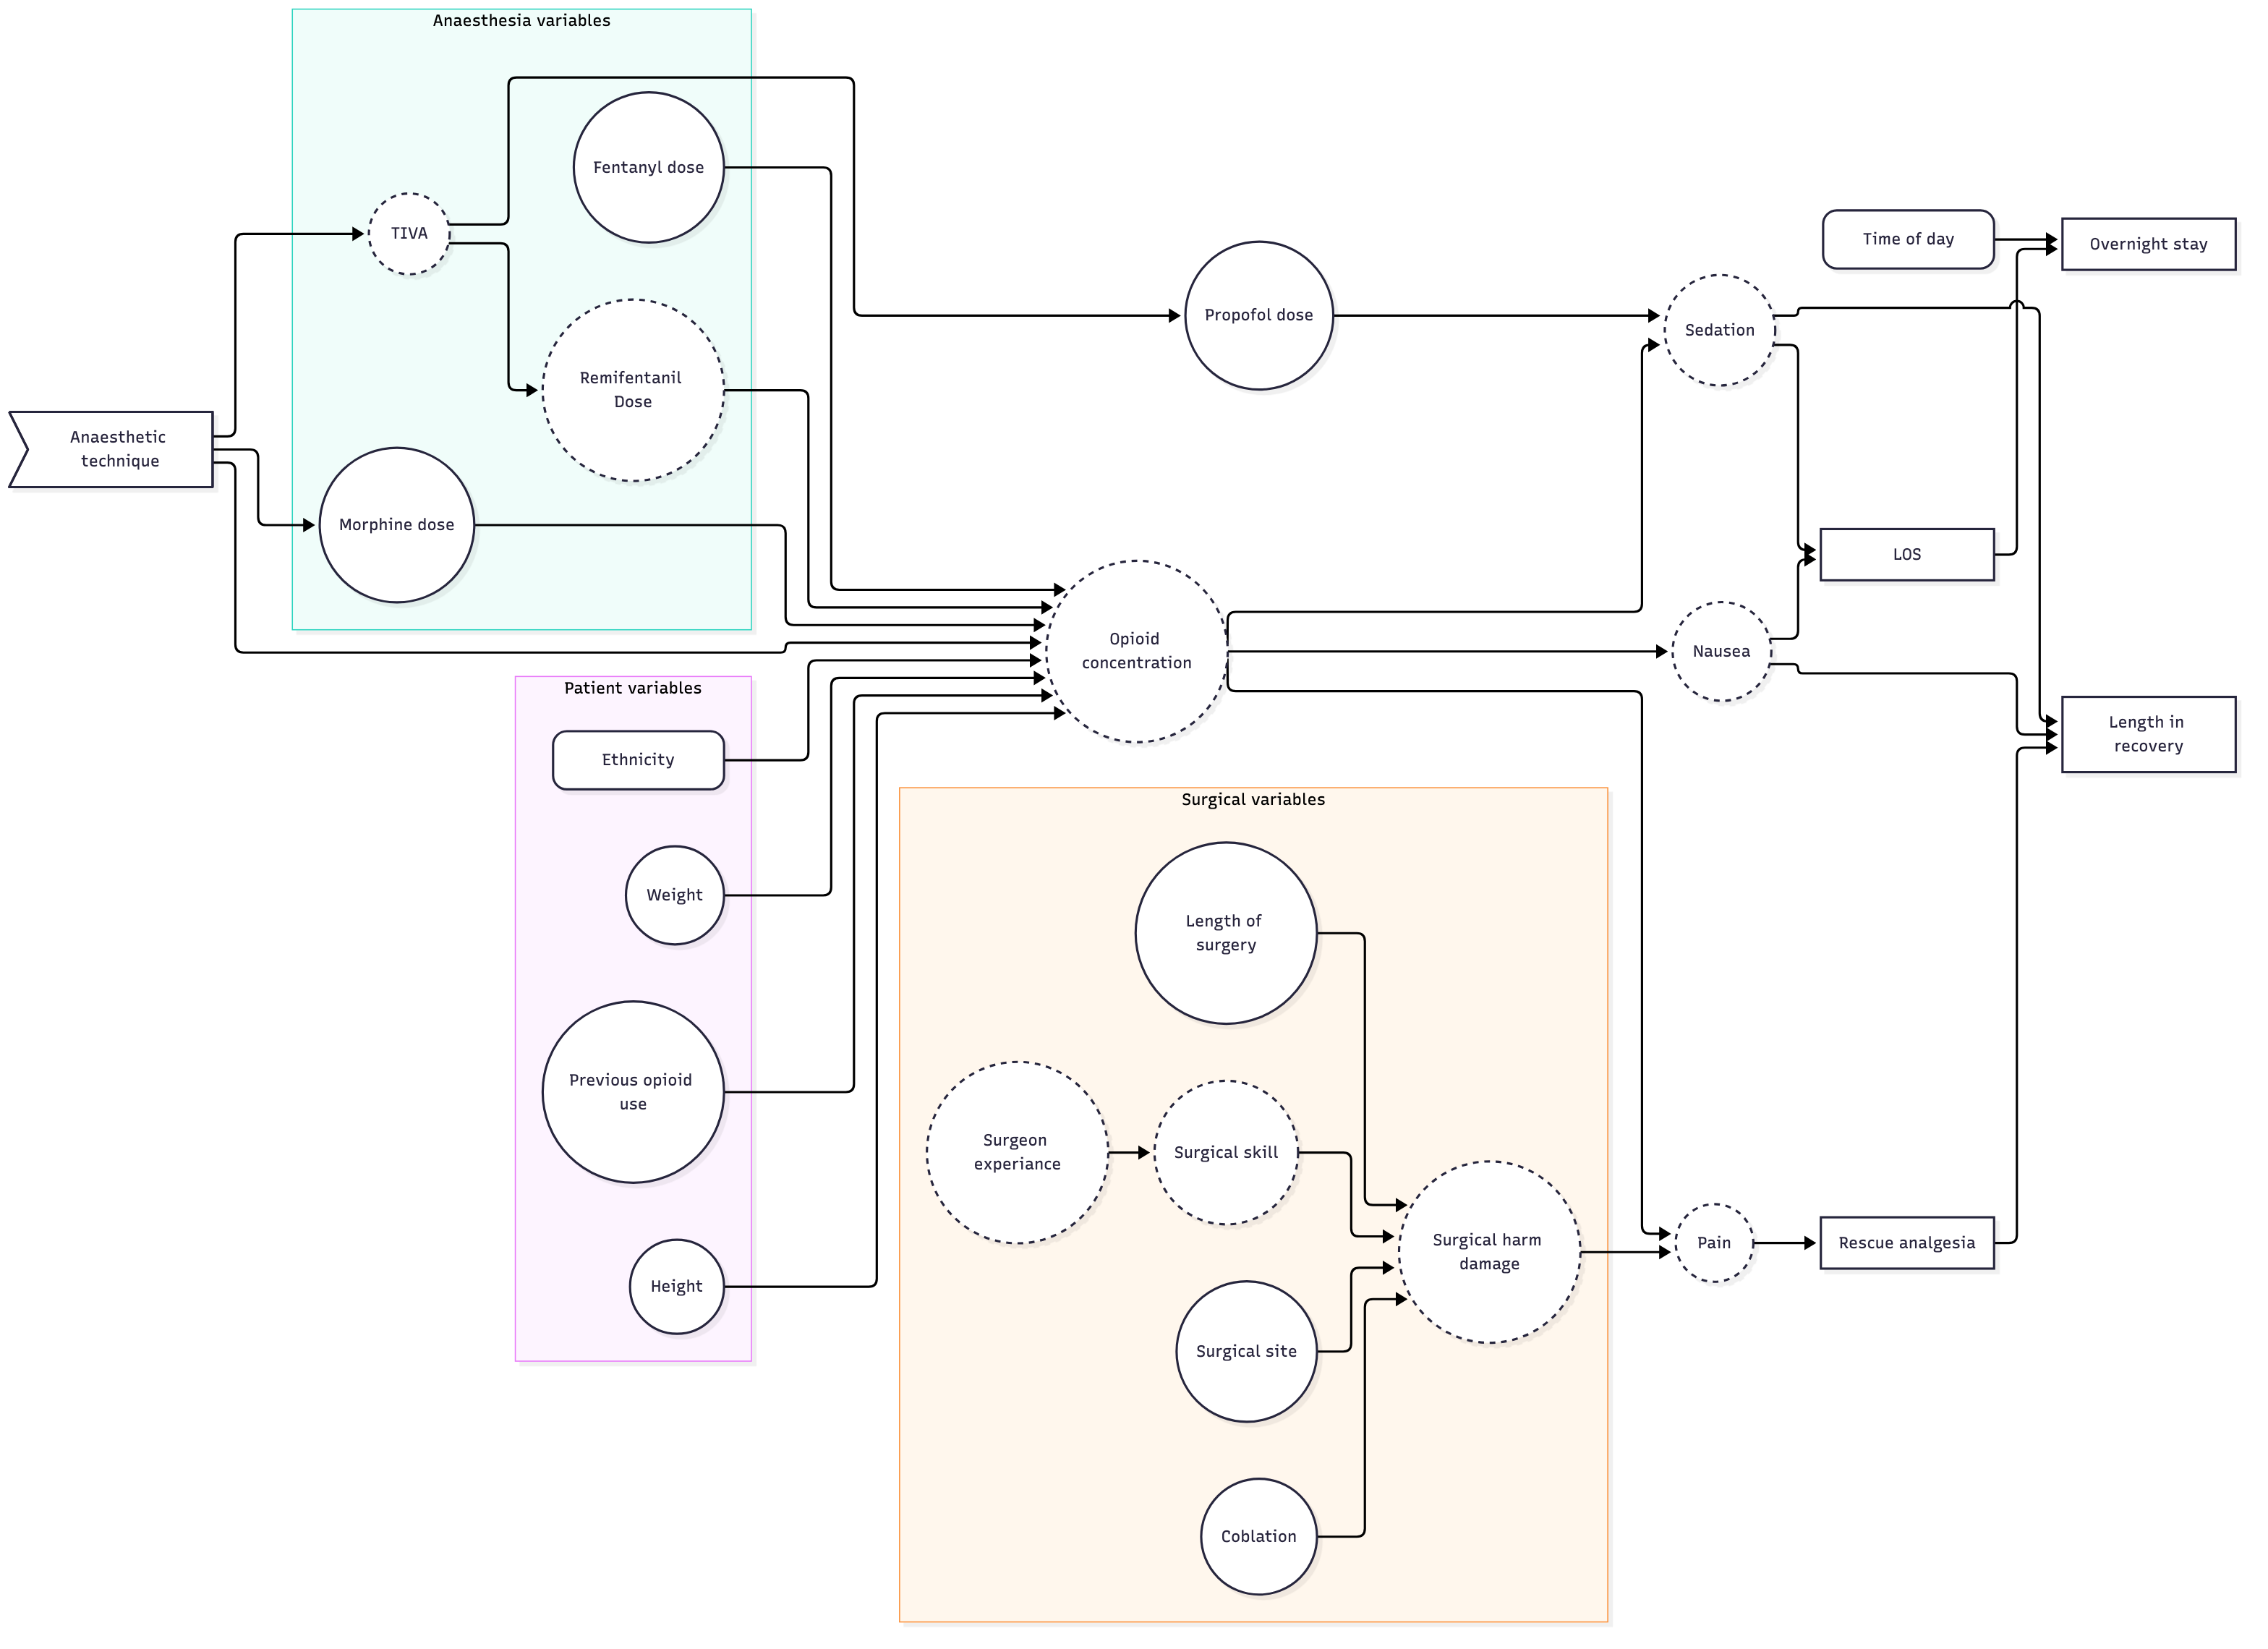
\includegraphics[keepaspectratio]{figures/sfig-dag.png}}

}

\caption{\label{sfig-dag}TODO: caption to be supplied by the authors.
(Old placeholder caption was: `A simple workflow diagram showing step A
leading to step B.')}

\end{sfig}%

\subsection{Models parameters}\label{sec-sm-model-parameters}

\begin{stbl}

\centering{

{\def\LTcaptype{none} % do not increment counter
\begin{longtable*}[]{@{}
  >{\raggedright\arraybackslash}p{(\linewidth - 10\tabcolsep) * \real{0.1667}}
  >{\raggedright\arraybackslash}p{(\linewidth - 10\tabcolsep) * \real{0.1667}}
  >{\raggedright\arraybackslash}p{(\linewidth - 10\tabcolsep) * \real{0.1667}}
  >{\raggedright\arraybackslash}p{(\linewidth - 10\tabcolsep) * \real{0.1667}}
  >{\raggedright\arraybackslash}p{(\linewidth - 10\tabcolsep) * \real{0.1667}}
  >{\raggedright\arraybackslash}p{(\linewidth - 10\tabcolsep) * \real{0.1667}}@{}}
\toprule\noalign{}
\begin{minipage}[b]{\linewidth}\raggedright
Model Number
\end{minipage} & \begin{minipage}[b]{\linewidth}\raggedright
Cohort
\end{minipage} & \begin{minipage}[b]{\linewidth}\raggedright
Outcome
\end{minipage} & \begin{minipage}[b]{\linewidth}\raggedright
Multi-level by primary anaesthetist
\end{minipage} & \begin{minipage}[b]{\linewidth}\raggedright
Co-variants
\end{minipage} & \begin{minipage}[b]{\linewidth}\raggedright
Notes
\end{minipage} \\
\midrule\noalign{}
\endhead
\bottomrule\noalign{}
\endlastfoot
0 & Adult & Recovery opioids & No & Nil & \\
1 & Adults & Recovery opioids & Yes & Nil & \\
2 & Adults & Recovery opioids & Yes & age, sex, surgical cohort, ASA,
history of chronic pain, procedure length and use of coblation & \\
3 & Adults & Time in recovery & Yes & & \\
4 & Adults & Same discharge & Yes & & \\
5 & Adults & Opioid on discharge & Yes & & Model fails to converge \\
6 & Adults & Return to ED at 7 days & Yes & & Model fails to converge \\
\end{longtable*}
}

}

\caption{\label{stbl-model-parameters}\textbf{TODO: caption to be
supplied by the authors.}}

\end{stbl}%

The following secondary outcomes were not modelled with the associated
justification:

\begin{itemize}
\item
  Length of admission (Days) -- Same day discharge has been modelled as
  a logistic regression instead due to the multi-modal disruption of
  length of admission.
\item
  Median pain score -- Significant number of missing data as pain scores
  not being collected in recovery, only on the ward.
\item
  Discharge medications -- Medication prescriptions at the point of
  discharge likely represent the variation in discharging clinician
  rather than anaesthetic clinician
\item
  Return to theatre-- Lack of distribution of outcome
\item
  Re-presentation -- Lack of distribution of outcome
\item
  Deaths -- Lack of distribution of outcome
\end{itemize}

\subsection{Multilevel modelling}\label{multilevel-modelling}

An ANOVA was performed between model 0 (without multi-level modelling)
and model 1 (with multi-level modelling) to establish the difference in
model performance

\begin{stbl}

\centering{

\begin{table}
\fontsize{12.0pt}{14.4pt}\selectfont
\begin{tabular*}{\linewidth}{@{\extracolsep{\fill}}rrrrrrrr}
\toprule
npar & AIC & BIC & logLik & deviance & Chisq & Df & Pr(>Chisq) \\ 
\midrule\addlinespace[2.5pt]
4 & 1297.392 & 1316.922 & -644.6960 & 1289.392 & NA & NA & NA \\ 
5 & 1297.667 & 1322.079 & -643.8336 & 1287.667 & 1.724714 & 1 & 0.1890873 \\ 
\bottomrule
\end{tabular*}
\end{table}

}

\caption{\label{stbl-model-anova}\textbf{ANOVA of Model 0 and Model 1.}}

\end{stbl}%

\subsection{Treatment group effects}\label{treatment-group-effects}

\begin{sfig}

\centering{

\pandocbounded{\includegraphics[keepaspectratio]{supplementary_materials_files/figure-pdf/chunk-sfig-forrest-plot-1.pdf}}

}

\caption{\label{sfig-forrest-plot}\textbf{Combined forest plots of
treatment group effect for outcome measures.} Left to right: 1)
unadjusted association between treatment group and rescue opioid
administration (model 1), 2) adjusted association between treatment
group and rescue opioid administration (model 2), 3) adjusted
association between treatment group and time spent in recovery, 4)
adjusted association between treatment group and same day discharge from
hospital.}

\end{sfig}%

\subsection{Results of Model 1}\label{sec-sm-model-1}

In Model 1 the variance explained by the anaesthetist ID was 5.0\%

\begin{stbl}

\centering{

\begin{table}
\caption*{
{\large } \\ 
{\small Cohort: Adult (unadjusted) Outcome: Recovery opioids}
} 
\fontsize{12.0pt}{14.4pt}\selectfont
\begin{tabular*}{\linewidth}{@{\extracolsep{\fill}}lrrrrrrr}
\toprule
Term & Coefficient & Standard error & z value & p value & Odds Ratio & OR 95\% CI Lower & OR 95\% CI Upper \\ 
\midrule\addlinespace[2.5pt]
(Intercept) & 0.546 & 0.228 & 2.400 & {\bfseries 0.0164} & 1.727 & 1.105 & 2.697 \\ 
Treatment group 2 & -0.111 & 0.260 & -0.425 & 0.6710 & 0.895 & 0.538 & 1.491 \\ 
Treatment group 3 & -0.064 & 0.244 & -0.261 & 0.7939 & 0.938 & 0.582 & 1.513 \\ 
Treatment group 4 & -1.262 & 0.276 & -4.580 & {\bfseries 0.0000} & 0.283 & 0.165 & 0.486 \\ 
\bottomrule
\end{tabular*}
\end{table}

}

\caption{\label{stbl-model-1-fixed}\textbf{Fixed effects of model 1.}}

\end{stbl}%

\begin{sfig}

\centering{

\pandocbounded{\includegraphics[keepaspectratio]{supplementary_materials_files/figure-pdf/chunk-sfig-model-1-random-1.pdf}}

}

\caption{\label{sfig-model-1-random}\textbf{Random effects of model 1.}}

\end{sfig}%

\subsection{Results of Model 2}\label{sec-sm-model-2}

In Model 1 the variance explained by the anaesthetist ID was 4.1\%

\begin{stbl}

\centering{

\begin{table}
\caption*{
{\large } \\ 
{\small Cohort: Adult (adjusted) Outcome: Recovery opioids}
} 
\fontsize{12.0pt}{14.4pt}\selectfont
\begin{tabular*}{\linewidth}{@{\extracolsep{\fill}}lrrrrrrr}
\toprule
Term & Coefficient & Standard error & z value & p value & Odds Ratio & OR 95\% CI Lower & OR 95\% CI Upper \\ 
\midrule\addlinespace[2.5pt]
(Intercept) & 1.035 & 0.345 & 2.998 & {\bfseries 0.0027} & 2.816 & 1.431 & 5.540 \\ 
Treatment group 2 & -0.062 & 0.347 & -0.180 & 0.8574 & 0.940 & 0.476 & 1.855 \\ 
Treatment group 3 & 0.130 & 0.338 & 0.385 & 0.6999 & 1.139 & 0.587 & 2.210 \\ 
Treatment group 4 & -0.872 & 0.490 & -1.779 & 0.0753 & 0.418 & 0.160 & 1.093 \\ 
Age (years) & -0.003 & 0.007 & -0.359 & 0.7194 & 0.997 & 0.984 & 1.011 \\ 
Sex: Male & -0.388 & 0.147 & -2.633 & {\bfseries 0.0085} & 0.678 & 0.508 & 0.906 \\ 
Cohort: Adenoidectomy & -0.972 & 0.283 & -3.434 & {\bfseries 0.0006} & 0.378 & 0.217 & 0.659 \\ 
Cohort: Adenotonsillectomy & -0.230 & 0.410 & -0.562 & 0.5742 & 0.794 & 0.356 & 1.774 \\ 
ASA: 2 & 0.186 & 0.149 & 1.247 & 0.2124 & 1.204 & 0.899 & 1.613 \\ 
ASA: 3 & 0.804 & 0.416 & 1.931 & 0.0535 & 2.234 & 0.988 & 5.051 \\ 
Chronic pain EPR diagnosis & 16.663 & 256.003 & 0.065 & 0.9481 & 17,246,029.420 & 0.000 & 1,402,715,160,700,723,036,991,085,236,294,291,222,509,907,398,686,037,744,012,270,541,774,420,156,692,178,477,797,837,346,132,154,155,918,370,517,607,311,201,282,249,445,059,944,771,087,740,661,532,664,219,839,845,972,394,937,020,114,226,193,982,581,458,489,460,882,747,848,551,010,650,420,099,940,352.000 \\ 
Procedure length (Minutes) & -0.002 & 0.003 & -0.661 & 0.5083 & 0.998 & 0.991 & 1.004 \\ 
Coblation & -1.049 & 0.398 & -2.636 & {\bfseries 0.0084} & 0.350 & 0.161 & 0.764 \\ 
Intra-operative opioid dose (OME mg) & -0.014 & 0.009 & -1.574 & 0.1154 & 0.986 & 0.969 & 1.003 \\ 
\bottomrule
\end{tabular*}
\end{table}

}

\caption{\label{stbl-model-2-fixed}\textbf{Fixed effects of model 2.}}

\end{stbl}%

\begin{sfig}

\centering{

\pandocbounded{\includegraphics[keepaspectratio]{supplementary_materials_files/figure-pdf/chunk-sfig-model-2-random-1.pdf}}

}

\caption{\label{sfig-model-2-random}\textbf{Random effects of model 2.}}

\end{sfig}%

\subsection{Results of Model 3}\label{sec-sm-model-3}

In Model 3 the standard deviation of the variance explained by the
anaesthetist ID was 2.33 minutes.

\begin{stbl}

\centering{

\begin{table}
\caption*{
{\large } \\ 
{\small Cohort: Adult (adjusted) Outcome: Time in recovery (minutes)}
} 
\fontsize{12.0pt}{14.4pt}\selectfont
\begin{tabular*}{\linewidth}{@{\extracolsep{\fill}}lrrrrrrr}
\toprule
Term & Coefficient & Standard error & z value & Degrees of freedom & p value & 95\% CI Lower & 95\% CI Upper \\ 
\midrule\addlinespace[2.5pt]
(Intercept) & 96.209 & 8.580 & 11.213 & 386.260 & {\bfseries 0.000} & 79.339 & 113.079 \\ 
Treatment group 2 & -15.384 & 8.725 & -1.763 & 584.869 & 0.078 & -32.520 & 1.753 \\ 
Treatment group 3 & -23.416 & 8.439 & -2.775 & 635.784 & {\bfseries 0.006} & -39.987 & -6.845 \\ 
Treatment group 4 & -42.086 & 12.534 & -3.358 & 733.664 & {\bfseries 0.001} & -66.692 & -17.479 \\ 
Age (years) & 0.100 & 0.178 & 0.563 & 915.766 & 0.574 & -0.249 & 0.450 \\ 
Sex: Male & -1.693 & 3.789 & -0.447 & 844.423 & 0.655 & -9.129 & 5.743 \\ 
Cohort: Adenoidectomy & -20.622 & 7.486 & -2.755 & 892.167 & {\bfseries 0.006} & -35.313 & -5.930 \\ 
Cohort: Adenotonsillectomy & -8.130 & 10.898 & -0.746 & 923.363 & 0.456 & -29.517 & 13.258 \\ 
ASA: 2 & 5.249 & 3.836 & 1.368 & 898.743 & 0.172 & -2.279 & 12.777 \\ 
ASA: 3 & 27.098 & 9.866 & 2.747 & 919.897 & {\bfseries 0.006} & 7.735 & 46.461 \\ 
Chronic pain EPR diagnosis & 5.969 & 27.232 & 0.219 & 924.724 & 0.827 & -47.475 & 59.414 \\ 
Procedure length (Minutes) & -0.012 & 0.086 & -0.136 & 920.494 & 0.892 & -0.181 & 0.157 \\ 
Coblation & 0.505 & 9.967 & 0.051 & 925.878 & 0.960 & -19.056 & 20.066 \\ 
Intra-operative opioid dose (OME mg) & 0.154 & 0.228 & 0.675 & 446.042 & 0.500 & -0.294 & 0.603 \\ 
\bottomrule
\end{tabular*}
\begin{minipage}{\linewidth}
p value's calculated using Satterthwaite's approximation \\
\end{minipage}
\end{table}

}

\caption{\label{stbl-model-3-fixed}\textbf{Fixed effects of model 3.}}

\end{stbl}%

\begin{sfig}

\centering{

\pandocbounded{\includegraphics[keepaspectratio]{supplementary_materials_files/figure-pdf/chunk-sfig-model-3-random-1.pdf}}

}

\caption{\label{sfig-model-3-random}\textbf{Random effects of model 3.}}

\end{sfig}%

\subsection{Results of Model 4}\label{sec-sm-model-4}

In Model 4 the variance explained by the anaesthetist ID was 25.2\%

\begin{stbl}

\centering{

\begin{table}
\caption*{
{\large } \\ 
{\small Cohort: Adult (adjusted) Outcome: Same day discharge}
} 
\fontsize{12.0pt}{14.4pt}\selectfont
\begin{tabular*}{\linewidth}{@{\extracolsep{\fill}}lrrrrrrr}
\toprule
Term & Coefficient & Standard error & z value & p value & Odds Ratio & OR 95\% CI Lower & OR 95\% CI Upper \\ 
\midrule\addlinespace[2.5pt]
(Intercept) & 1.794 & 0.409 & 4.389 & {\bfseries 0.0000} & 6.011 & 2.699 & 13.391 \\ 
Treatment group 2 & 0.820 & 0.409 & 2.007 & {\bfseries 0.0448} & 2.271 & 1.019 & 5.059 \\ 
Treatment group 3 & 0.611 & 0.395 & 1.548 & 0.1217 & 1.843 & 0.850 & 3.998 \\ 
Treatment group 4 & 1.155 & 0.610 & 1.894 & 0.0582 & 3.173 & 0.961 & 10.482 \\ 
Age (years) & -0.002 & 0.008 & -0.192 & 0.8474 & 0.998 & 0.982 & 1.015 \\ 
Sex: Male & -0.371 & 0.178 & -2.081 & {\bfseries 0.0375} & 0.690 & 0.487 & 0.979 \\ 
Cohort: Adenoidectomy & 1.278 & 0.420 & 3.041 & {\bfseries 0.0024} & 3.588 & 1.575 & 8.177 \\ 
Cohort: Adenotonsillectomy & -0.014 & 0.492 & -0.029 & 0.9768 & 0.986 & 0.376 & 2.585 \\ 
ASA: 2 & -0.338 & 0.185 & -1.829 & 0.0674 & 0.713 & 0.496 & 1.025 \\ 
ASA: 3 & -1.646 & 0.412 & -3.998 & {\bfseries 0.0001} & 0.193 & 0.086 & 0.432 \\ 
Chronic pain EPR diagnosis & -0.018 & 1.194 & -0.015 & 0.9880 & 0.982 & 0.095 & 10.192 \\ 
Procedure length (Minutes) & -0.018 & 0.004 & -4.538 & {\bfseries 0.0000} & 0.982 & 0.975 & 0.990 \\ 
Coblation & 0.310 & 0.566 & 0.548 & 0.5838 & 1.364 & 0.449 & 4.139 \\ 
Intra-operative opioid dose (OME mg) & 0.000 & 0.011 & -0.024 & 0.9810 & 1.000 & 0.978 & 1.022 \\ 
\bottomrule
\end{tabular*}
\end{table}

}

\caption{\label{stbl-model-4-fixed}\textbf{Fixed effects of model 4.}}

\end{stbl}%

\begin{sfig}

\centering{

\pandocbounded{\includegraphics[keepaspectratio]{supplementary_materials_files/figure-pdf/chunk-sfig-model-4-random-1.pdf}}

}

\caption{\label{sfig-model-4-random}\textbf{Random effects of model 4.}}

\end{sfig}%

\subsection{Results of Model 5}\label{sec-sm-model-5}

In Model 5 the variance explained by the anaesthetist ID was 0.0\%

\begin{stbl}

\centering{

\begin{table}
\caption*{
{\large } \\ 
{\small Cohort: Adult (adjusted) Outcome: Opioids on discharge}
} 
\fontsize{12.0pt}{14.4pt}\selectfont
\begin{tabular*}{\linewidth}{@{\extracolsep{\fill}}lrrrrrrr}
\toprule
Term & Coefficient & Standard error & z value & p value & Odds Ratio & OR 95\% CI Lower & OR 95\% CI Upper \\ 
\midrule\addlinespace[2.5pt]
(Intercept) & -24.131 & 11,747.732 & -0.002 & 0.9984 & 0.000 & 0.000 &  Inf \\ 
Treatment group 2 & 18.902 & 11,747.732 & 0.002 & 0.9987 & 161,872,469.179 & 0.000 &  Inf \\ 
Treatment group 3 & 18.763 & 11,747.732 & 0.002 & 0.9987 & 140,889,946.846 & 0.000 &  Inf \\ 
Treatment group 4 & 18.443 & 11,747.732 & 0.002 & 0.9987 & 102,260,208.641 & 0.000 &  Inf \\ 
Age (years) & 0.054 & 0.032 & 1.676 & 0.0937 & 1.055 & 0.991 & 1.124 \\ 
Sex: Male & -1.268 & 1.085 & -1.168 & 0.2428 & 0.282 & 0.034 & 2.362 \\ 
Cohort: Adenoidectomy & -35.426 & 8,108,195.936 & 0.000 & 1.0000 & 0.000 & 0.000 &  Inf \\ 
Cohort: Adenotonsillectomy & -37.725 & 13,013,560.905 & 0.000 & 1.0000 & 0.000 & 0.000 &  Inf \\ 
ASA: 2 & -1.220 & 0.913 & -1.337 & 0.1812 & 0.295 & 0.049 & 1.766 \\ 
ASA: 3 & -45.321 & 11,447,390.845 & 0.000 & 1.0000 & 0.000 & 0.000 &  Inf \\ 
Chronic pain EPR diagnosis & -35.964 & 33,676,253.936 & 0.000 & 1.0000 & 0.000 & 0.000 &  Inf \\ 
Procedure length (Minutes) & 0.006 & 0.021 & 0.282 & 0.7780 & 1.006 & 0.966 & 1.047 \\ 
Coblation & -33.222 & 12,121,752.973 & 0.000 & 1.0000 & 0.000 & 0.000 &  Inf \\ 
Intra-operative opioid dose (OME mg) & -0.015 & 0.046 & -0.319 & 0.7497 & 0.985 & 0.901 & 1.078 \\ 
\bottomrule
\end{tabular*}
\end{table}

}

\caption{\label{stbl-model-5-fixed}\textbf{Fixed effects of model 5.}}

\end{stbl}%

\begin{sfig}

\centering{

\pandocbounded{\includegraphics[keepaspectratio]{supplementary_materials_files/figure-pdf/chunk-sfig-model-5-random-1.pdf}}

}

\caption{\label{sfig-model-5-random}\textbf{Random effects of model 5.}}

\end{sfig}%

\subsection{Results of Model 6}\label{sec-sm-model-6}

In Model 6 the variance explained by the anaesthetist ID was 6.7\%

\begin{stbl}

\centering{

\begin{table}
\caption*{
{\large } \\ 
{\small Cohort: Adult (adjusted) Outcome: Presentation to emergency department within 7 days}
} 
\fontsize{12.0pt}{14.4pt}\selectfont
\begin{tabular*}{\linewidth}{@{\extracolsep{\fill}}lrrrrrrr}
\toprule
Term & Coefficient & Standard error & z value & p value & Odds Ratio & OR 95\% CI Lower & OR 95\% CI Upper \\ 
\midrule\addlinespace[2.5pt]
(Intercept) & -1.251 & 0.495 & -2.526 & {\bfseries 0.0115} & 0.286 & 0.108 & 0.755 \\ 
Treatment group 2 & -0.019 & 0.496 & -0.038 & 0.9695 & 0.981 & 0.371 & 2.592 \\ 
Treatment group 3 & 0.039 & 0.483 & 0.081 & 0.9356 & 1.040 & 0.403 & 2.682 \\ 
Treatment group 4 & -0.658 & 0.721 & -0.912 & 0.3616 & 0.518 & 0.126 & 2.129 \\ 
Age (years) & -0.018 & 0.011 & -1.699 & 0.0893 & 0.982 & 0.962 & 1.003 \\ 
Sex: Male & 0.100 & 0.213 & 0.467 & 0.6406 & 1.105 & 0.727 & 1.678 \\ 
Cohort: Adenoidectomy & -1.479 & 0.623 & -2.376 & {\bfseries 0.0175} & 0.228 & 0.067 & 0.772 \\ 
Cohort: Adenotonsillectomy & -1.460 & 1.032 & -1.415 & 0.1572 & 0.232 & 0.031 & 1.756 \\ 
ASA: 2 & 0.047 & 0.207 & 0.226 & 0.8214 & 1.048 & 0.699 & 1.572 \\ 
ASA: 3 & -0.734 & 0.760 & -0.966 & 0.3339 & 0.480 & 0.108 & 2.127 \\ 
Chronic pain EPR diagnosis & 0.885 & 1.198 & 0.739 & 0.4599 & 2.424 & 0.232 & 25.375 \\ 
Procedure length (Minutes) & 0.000 & 0.005 & 0.004 & 0.9968 & 1.000 & 0.990 & 1.010 \\ 
Coblation & -14.444 & 362.041 & -0.040 & 0.9682 & 0.000 & 0.000 & 78,822,125,137,534,361,928,301,625,501,438,453,285,514,137,540,345,737,809,912,876,469,785,903,132,926,720,178,742,846,887,992,591,595,491,155,192,313,195,174,792,047,902,159,847,274,472,471,453,547,011,572,751,347,387,568,453,607,950,986,566,774,657,066,017,152,467,242,072,639,781,306,646,785,239,564,482,895,420,554,450,246,068,414,540,706,707,615,436,296,314,379,785,492,258,673,554,435,631,742,976.000 \\ 
Intra-operative opioid dose (OME mg) & 0.002 & 0.013 & 0.163 & 0.8707 & 1.002 & 0.977 & 1.027 \\ 
\bottomrule
\end{tabular*}
\end{table}

}

\caption{\label{stbl-model-6-fixed}\textbf{Fixed effects of model 6.}}

\end{stbl}%

\begin{sfig}

\centering{

\pandocbounded{\includegraphics[keepaspectratio]{supplementary_materials_files/figure-pdf/chunk-sfig-model-6-random-1.pdf}}

}

\caption{\label{sfig-model-6-random}\textbf{Random effects of model 6.}}

\end{sfig}%




\end{document}
